\documentclass{sig-alternate-05-2015}
 
\pagenumbering{arabic} % Remove for camera-ready

\makeatletter
\setcounter{tocdepth}{3}
\def\contentsname{Contents}
\def\tableofcontents{%
    \section*{\MakeUppercase{\contentsname}}%
    \@starttoc{toc}%
    }
\makeatother

\newcommand{\TITLE}{Cloud Metrics for Academic Resource Providers for Research and Education}

\newcommand{\AUTHOR}{ Gregor von Laszewski, Hyungro Lee, Fugang Wang} 

%\iCHART \HS
%\iCHARTS \HS
%\iDISPLAY \HS
%\iTABLE \HS
%\iSTAT \HS
%\iCHARTS \HS
%\iFILE \HS
%\iFILES \HS
%\iCLUSTER \HS


\newenvironment{fTREE}[1]
    {   \begin{center}
        \begin{tiny}
        \begin{tikzpicture}[grow'=right,level distance=#1,
                                      sibling distance=.0in,anchor=west,child anchor=west, ]
                  \tikzset{edge from parent/.style= 
                    {draw, edge from parent fork right}}
}
    {\end{tikzpicture}
     \end{tiny}
     \end{center}
}

%%%%%%%%%%%%%%%%%%%%%%%%%%%%%%%%%%%%%%%%%%%%%%%%%%%%%%%%%%%%%%

% LATEX DEFINITIONS 
%%%%%%%%%%%%%%%%%%%%%%%%%%%%%%%%%%%%%%%%%%%%%%%%%%%%%%%%%%%%%%

\usepackage[colorlinks]{hyperref}
\usepackage{array} 
\usepackage{graphicx} 
\usepackage{booktabs} 
\usepackage{pifont} 
\usepackage[colorinlistoftodos]{todonotes}
\usepackage{rotating} 
\usepackage{color} 
\usepackage{listings}
\usepackage{enumitem}
\usepackage{fancyvrb}
\usepackage{colortbl}
%\usepackage{longtable}
%\usepackage{tabularx}
\usepackage{booktabs}
\usepackage{array}
%\usepackage{supertabular}
%\usepackage{multicol}
%\usepackage{tabu}
\usepackage{afterpage}
%\usepackage{pdflscape}
\usepackage{xtab}

\usepackage{tikz}
\usepackage{tikz-qtree}
\usetikzlibrary{trees,shapes,arrows}
\usepackage{dot2texi}
\usepackage{graphviz}

%\usepackage{forest}
%\usepackage{float}
%\usepackage{afterpage}

\newcommand*\rot{\rotatebox{90}} 
 
%\newcommand{\FILE}[1]{\todo[color=green!40]{#1}} 

\newcommand{\fugang}[1]{\todo[inline, color=orange!20]{~#1}} 
\newcommand{\hyungro}[1]{\todo[inline, color=green!20]{~#1}} 
\newcommand{\gregor}[1]{\todo[inline, color=blue!20]{~#1}} 
\newcommand{\task}[1]{\smallskip\todo[inline, color=gray!20]{#1}} 
\newcommand{\improve}[1]{\smallskip\todo[inline, color=gray!20]{old: #1}} 

%\setlist[itemize]{noitemsep, topsep=0pt} 
%%%%%%%%%%%%%%%%%%%%%%%%%%%%%%%%%%%%%%%%%%%%%%%%%%%%%%%%%%%%%%
% HYPERSETUP 
%%%%%%%%%%%%%%%%%%%%%%%%%%%%%%%%%%%%%%%%%%%%%%%%%%%%%%%%%%%%%%

\hypersetup{ 
    bookmarks=true,         % show bookmarks bar 
    unicode=false,          % non-Latin characters in Acrobat’s bookmarks 
    pdftoolbar=true,        % show Acrobat’s toolbar 
    pdfmenubar=true,        % show Acrobat’s menu 
    pdffitwindow=false,     % window fit to page when opened 
    pdfstartview={FitH},    % fits the width of the page to the window 
    pdftitle={\TITLE},    % title 
    pdfauthor={\AUTHOR},     % author 
    pdfsubject={Subject},   % subject of the document 
    pdfcreator={Gregor von Laszewski, Fugang Wang},   % creator of the document 
    pdfproducer={Gregor von Laszewski}, % producer of the document 
    pdfkeywords={hindex} {metric}{FutureGrid}, % list of keywords 
    pdfnewwindow=true,      % links in new window 
    colorlinks=false,       % false: boxed links; true: colored links 
    linkcolor=red,          % color of internal links (change box color with linkbordercolor) 
    citecolor=green,        % color of links to bibliography 
    filecolor=magenta,      % color of file links 
    urlcolor=cyan           % color of external links 
} 
 
%%%%%%%%%%%%%%%%%%%%%%%%%%%%%%%%%%%%%%%%%%%%%%%%%%%%%%%%%%%%%%%%%%%%%% 



\lstset{frame=tb,
language=sh,
aboveskip=3mm,
belowskip=3mm,
showstringspaces=false,
columns=flexible,
basicstyle={\scriptsize\ttfamily},
numbers=none,
numberstyle=\tiny\color{gray},
keywordstyle=\color{blue},
commentstyle=\color{dkgreen},
stringstyle=\color{mauve},
breaklines=true,
breakatwhitespace=true
tabsize=3
}

\newcommand{\iCHART}{
\includegraphics[scale=0.3]{icons/glyphicons-43-pie-chart.png}}
\newcommand{\iDISPLAY}{
\includegraphics[scale=0.3]{icons/glyphicons-87-display.png}}
\newcommand{\iTABLE}{
\includegraphics[scale=0.3]{icons/glyphicons-120-table.png}}
\newcommand{\iSTAT}{
\includegraphics[scale=0.3]{icons/glyphicons-41-stats.png}}
\newcommand{\iCHARTS}{
\includegraphics[scale=0.3]{icons/glyphicons-42-charts.png}}
\newcommand{\iFILE}{
\includegraphics[scale=0.3]{icons/glyphicons-37-file.png}}
\newcommand{\iFILES}{
\includegraphics[scale=0.3]{icons/glyphicons-319-more-items.png}}
\newcommand{\iCLUSTER}{
\includegraphics[scale=0.3]{icons/glyphicons-508-cluster.png}}
\newcommand{\HS}{\hspace{1pt}}


%\renewcommand\floatpagefraction{.9}
%\renewcommand\topfraction{.9}
%\renewcommand\bottomfraction{.9}
%\renewcommand\textfraction{.1}   
%\setcounter{totalnumber}{50}
%\setcounter{topnumber}{50}
%\setcounter{bottomnumber}{50}

\begin{document} 
% 
% --- Author Metadata here --- 
\conferenceinfo{Report}{Permission to make digital or hard copies of all or part of this work for personal or classroom use is granted without fee provided that copies are not made or distributed for profit or commercial advantage and that copies bear this notice and the full citation on the first page. To copy otherwise, or republish, to post on servers or to redistribute to lists, requires prior specific permission and/or a fee.
%SAC’10, March 22-26, 2010, Sierre, Switzerland.
%Copyright 2010 ACM 978-1-60558-638-0/10/03…\$10.00.
}
\CopyrightYear{2015}  
\crdata{X-XXXXX-XX-X/XX/XX}  % Allows default copyright data (0-89791-88-6/97/05) to be over-ridden - IF NEED BE. 
% --- End of Author Metadata --- 
 
\title{\TITLE} 
%\subtitle{[Extended Abstract] 
\titlenote{A current draft version of this paper is available at \\
{\tiny\texttt{https://github.com/cyberaide/paper-metric/blob/master/vonLaszewski-metric-draft.pdf}}}
 
\numberofauthors{1}

\author{ 
\alignauthor
Gregor  von Laszewski $^1$\titlenote{Corresponding Author.}, Hyungro Lee$^1$, Fugang Wang$^1$, Geoffrey C. Fox$^1$, \\
Thomas Furlani$^2$, Robert DeLeon$^2$, Qiao Chunming$^2$\\
       \smallskip
       \affaddr{$^1$Indiana University, 2719 10th Street, Bloomington, Indiana, U.S.A.}\\ 
       \affaddr{$^2$SUNY at Buffalo, 701 Ellicott Street, Buffalo, New York, 14203, U.S.A.}\\ 
       \smallskip\email{$^*$laszewski@gmail.com} 
}
\date{24 March 2014}  

\newpage 
{\flushleft\bf \TITLE}
\tableofcontents

\newpage
\listoftodos[Notes]
\newpage
\toappear{} 
\maketitle 
\begin{abstract} 

Cloud computing has established itself as one of the key components in modern datacenters. Such datacenter include not only government and for profit organizations but also academic institutions. One of the important aspects to a successfully operate and utilize clouds in any organization is the availability of sophisticated metric information and frameworks to assure a number of key operational factors are met that are measured by such metrics. In this paper we provide an overview of the different aspects that are shaping the need for cloud metrics. We especially identify the needs for cloud metrics and monitoring solutions for various user communities that are an important factor for academic cloud providers. Application users, administrators, academic and funders shape the motivation for academic cloud metrics.  Metrics of interest support usage monitoring, failure and auditing data to identify user and system behavior. The information needs to be gathered as a mashup and exposed conveniently to the users as API, command tools, and a portal with charting capability, as well as periodically generated customizable reports. Many of the metrics presented, have been successfully used as part of the FutureGrid and FutureSystems clouds. This includes also the unified metrics service framework allowing integration of metrics from heterogeneous clouds such as OpenStack, Eucalyptus and Nimbus. Additionally, we see the importance of metrics also to be used as part of higher-level platform as a service and SaaS that utilize underlying IaaS. Thus it is important to identify additional features of existing and future services that benefit from metrics and their exposure to its users within the cloud context.

\end{abstract} 

% %%%%%%%%%%%%%%%%%%%%%%%%%%%%%%%%%%%%%%%%%%%%%%%%%%%%%%%%%%%%%%%%%%%%%%
% ACM CLASSIFICATION, Terms, Keywords,
% %%%%%%%%%%%%%%%%%%%%%%%%%%%%%%%%%%%%%%%%%%%%%%%%%%%%%%%%%%%%%%%%%%%%%%
\begin{CCSXML}
<ccs2012>
<concept>
<concept_id>10002944.10011123.10011124</concept_id>
<concept_desc>General and reference~Metrics</concept_desc>
<concept_significance>500</concept_significance>
</concept>
<concept>
<concept_id>10003033.10003099.10003100</concept_id>
<concept_desc>Networks~Cloud computing</concept_desc>
<concept_significance>500</concept_significance>
</concept>
</ccs2012>
\end{CCSXML}

\ccsdesc[500]{Networks~Cloud computing}
\ccsdesc[500]{General and reference~Metrics}

\printccsdesc

\keywords{Cloud Metrics, Resource Monitoring, Cloud Accounting, Metering, FutureGrid, FutureSystems, XSEDE} 

%%%%%%%%%%%%%%%%%%%%%%%%%%%%%%%%%%%%%%%%%%%%%%%%%%%%%%%%%%%%%%%%%%%%%% 
% SECTIONS 
%%%%%%%%%%%%%%%%%%%%%%%%%%%%%%%%%%%%%%%%%%%%%%%%%%%%%%%%%%%%%%%%%%%%%% 

%%%%%%%%%%%%%%%%%%%%%%%%%%%%%%%%%%%%%%%%%%%%%%%%%%%%%%%%%%%%%%%%%%%%%%
\section{INTRODUCTION}
%%%%%%%%%%%%%%%%%%%%%%%%%%%%%%%%%%%%%%%%%%%%%%%%%%%%%%%%%%%%%%%%%%%%%%

Cloud computing has established itself as one of the key components in modern datacenters. This includes academic, government, and for profit institutions and organizations.  According to the NIST definition ``Cloud computing is a model for enabling ubiquitous, convenient, on-demand network access to a shared pool of configurable computing resources (e.g., networks, servers, storage, applications, and services) that can be rapidly provisioned and released with minimal management effort or service provider interaction''~\cite{mell2011nist}. Essential characteristics include on-demand self-service, broad network access, rapid elasticity, and measured service. Important service models are Software as a Service (SaaS), Platform as a Service (PaaS), and Infrastructure as a Service (IaaS). Deployments include private clouds, community clouds, public clouds, and hybrid clouds.

Academic cloud computing has become an important resource in universities and institutions. One of the important aspects to successfully operate and offer cloud services is the availability of sophisticated metric information and frameworks assuring that a number of key operational factors are met. As cloud computing is typically part of a large-scale datacenter it also integrates common data center and service metrics. Thus it is not sufficient to just provide virtual machine related information but work towards a comprehensive integrated data framework that supports the creation of meaningful metrics through a sophisticated data mashup. Hence it is important to analyze and describe the requirements from metric frameworks and provide concrete ideas about which metrics and services are to be provided in order to support academic cloud computing.


The rest of the paper is structured as follows. First we define what academic cloud computing comprises. In Section~\ref{S:factors} we introduce some major factors that need to be considered when providing a cloud monitoring and metric framework. We introduce some concrete metrics in Section~\ref{S:metrics}.  A brief summary of monitoring tools and services is provided in Section~\ref{S:tools}.  Section~\ref{S:cloudmesh} showcases our hybrid cloud monitoring and metrics services that have been used in FutureGrid and are currently used in FutureSystems. Related activities are briefly summarized in Section~\ref{S:related}.  We conclude our paper while summarizing our findings in Section~\ref{S:conclusion}.

\section{ACADEMIC CLOUD COMPUTING}
\label{S:academiccc}

Academic cloud computing offers to the academic community a variety of clouds to a very diverse user community. In contrast to commercial offerings some of them have some unique properties that explicitly target the academic user communities. On the one hand it includes clouds offered by the universities or institutions IT organization in support of production level services. This may include e-mail, calendars, and document sharing environments, accounting and the organizations Web presence. Recently, such services are increasingly offered through outsourcing by utilizing public clouds or services. The demand for such service offerings are typically not different from any other large organization running operational production services of large organizations. On the other hand institutions and universities are in the need to provide a wide variety of sophisticated infrastructure, services, and platforms to the academic {\it research} and {\it education} community. It is also not sufficient to just provide the services but to provide a {\em testbed as a service (TaaS)} allowing the services to become part of the research conducted within the organization. Hence, infrastructure, platform, and software as a service frameworks become itself a target of research as demonstrated by the FutureGrid project. In addition we find typical development resources needed in support of disciplines utilizing computer and computational science. Figure~\ref{TAX:academic} depicts the various groups. In this paper we will ignore the IT production environments as they are similar to commercial clouds and focus on the clouds needed to support the research agenda of the academic community.

\begin{figure}[htb]
\begin{fTREE}{1.1in}  \Tree
     [. {Academic Cloud}
        [. Production
            [. e-mail ]
            [. {Web presence} ]
            [. {Operational Services} ]	
            [. {Course management} ]
        ]	
	[. {Education \& Research}
		[. {Development} ]      
           	[. {Testbed} ]               
		 [. {Computational Services} ]        
        ]
   ]
\end{fTREE}
\vspace{-12pt}
\caption{Academic cloud computing applications.}
\label{TAX:academic}
 \end{figure}
 
Within the offerings to the academic research and education community we observe not only the usage of private clouds but also the usage of public clouds. Furthermore, traditional high performance computing (HPC) is offered as a platform in many organizations and allows to support the paradigm of {\it HPC in the cloud} as showcased for example by the Extreme Science and Engineering Discovery Environment (XSEDE) project (see Section~\ref {S:resources} for more details).  It validates that HPC as a service is established not only as part of the academic offerings, but also by commercial offerings as demonstrated by Amazon High Performance Computing~\cite{awshpc}, IBM Platform Computing~\cite{ibmhpc}, and with additional examples provided in~\cite{DouglasEadline}. Through this interplay we find a convergence of Clouds, Grids, HPC, and Utility Computing into a computational service mesh that we have explored as part of our cloudmesh activities \cite{las14cloudmeshmultiple, las12fg-bookchapter}. Metrics in regards to HPC have been described in sufficient detail in \cite{las13xdmod} and are listed in the appendix of this paper (see \ref{??}).



\subsection{Cloud Metrics}

In order to support the effort of academic cloud computing we answer the following questions as part of this paper:

\begin{enumerate}
\setlength\itemsep{-2pt}
\item Which metrics are useful for whom and why? (Section~\ref{S:metrics})
\item Which community is targeted? (Section~\ref{S:academiccc})
\item Which services are targeted? (Section~\ref{??})
\item Which resources are monitored? (Section~\ref{??})
\item What privacy aspects exist? (Section~\ref{??})
\item Which metric efforts exists? (Section~\ref{S:related})
\end{enumerate}

Academic cloud metrics are important to a number of academic users interested in the various aspects dealing with development, operation, use, and management of a cloud. Hence, the motivation for cloud metrics are shaped by application users, administrators, service providers and funders. Basic metrics include usage, failure and auditing data to identify user and system behavior. Many of the metrics presented here have been used as part of the FutureGrid and FutureSystems clouds. These general aspects are not only common to a particular IaaS framework but are common across heterogeneous cloud IaaS such as OpenStack, Eucalyptus and Nimbus including unified metrics across such deployments. Even within a single IaaS framework we see multiple versioned deployments and customized versions as part of test beds and development environments. 

Additionally, we metrics play an important role as part of offering higher-level platforms and software to support user communities benefitting from them. Thus it is important to identify common features of existing and future services that benefit from metrics and their exposure to its users. 

\subsection{Unique Academic Requirements}

In some areas there is no fundamental distinction for metrics between academic and non-academic resource providers. Areas where there exists distinction are metrics based on charging models, and the utilization of hybrid clouds. Furthermore, we find that higher level metrics and metrics integrating into other frameworks provided as PaaS and HPC frameworks. An isolated inspection of the data associated with basic metrics may not be sufficient.

The reason for this is that some projects may require a combination of technologies that motivate project wide metrics to not only display usage and utilization of the various frameworks but also the associated high-level services. Examples include pooling of heterogeneous resources and services providing a {\it computational mesh} while at the same time going potentially beyond the concepts of utilization of cloud, HPC, and Grid computing. Due to the limited resources in academic organizations we also often do not have (in contrast to public clouds) an ``unlimited�� resource pool. For example the XSEDE resources receive resource requests that are four times higher than the available resources. Hence, it is important to identify performance metrics and benchmarks that lead to an improvement of the applications using such resources. For academic cloud resources availability and scalability also need to be ensured to manage rapid changes (which we see for example in educational usage patterns as part of classes) in the demands for cloud resources. However, performance metrics my be including ease of use and time to deployment rather than just hardware resource characteristics. Typical factors when considering performance analysis and monitoring applied to cloud computing include (a) performance isolation against interference (b) availability and scalability (c) cost effectiveness to fully utilize available resources.

As other clouds academic clouds rely on sharing of the offered services. However, just as in public clouds many users may not understand the implication and cost that is prevalent when using a particular service. Hence detailed metrics informing the user not only at time of an experiment, but access to information that helps planning such experiments are needed. Thus metrics will address and provide an essential input to several concrete challenges for academic clouds to understand the reliability, status, and behavior of underlying resources and services which are typically not provided in sufficient detail by public clouds. In some applications of clouds we also see differentiations in the need for privacy. For example in XSEDE the data available on a per project base is typically not accessible in public clouds de to the open nature of funding.

%%%%%%%%%%%%%%%%%%%%%%%%%%%%%%%%%%%%%%%%%%%%%%%%%%%%%%%%%%%%%%%%%%%%%%
\section{CLOUD METRIC FACTORS} \label {S:factors}
%%%%%%%%%%%%%%%%%%%%%%%%%%%%%%%%%%%%%%%%%%%%%%%%%%%%%%%%%%%%%%%%%%%%%%

When we look at a particular cloud metric, it may be shaped by a number of factors that determines the applicability and usability of the metric in general. To provide an overview of a selected number of factors fro cloud metrics we have identified the following factors of significant importance: (a) stakeholders and roles to address, (b) the frameworks to address, (c) the purpose the metrics are designed for, (d) concrete resources are targeted by the metric, (e) which sources are used for the metric, and (f) which security aspects are considered. We are summarizing these influential aspects in Figure \ref{F:taxonomy-1}\footnote{We will update the Figure \ref{F:taxonomy-1} in the final version of the paper. For now it shows a subset of information as presented in the subsections according the important factors discussed within this paper.} and explaining them in more detail in the subsequent sections.

\begin{figure}[!h] 
  {\centering 
    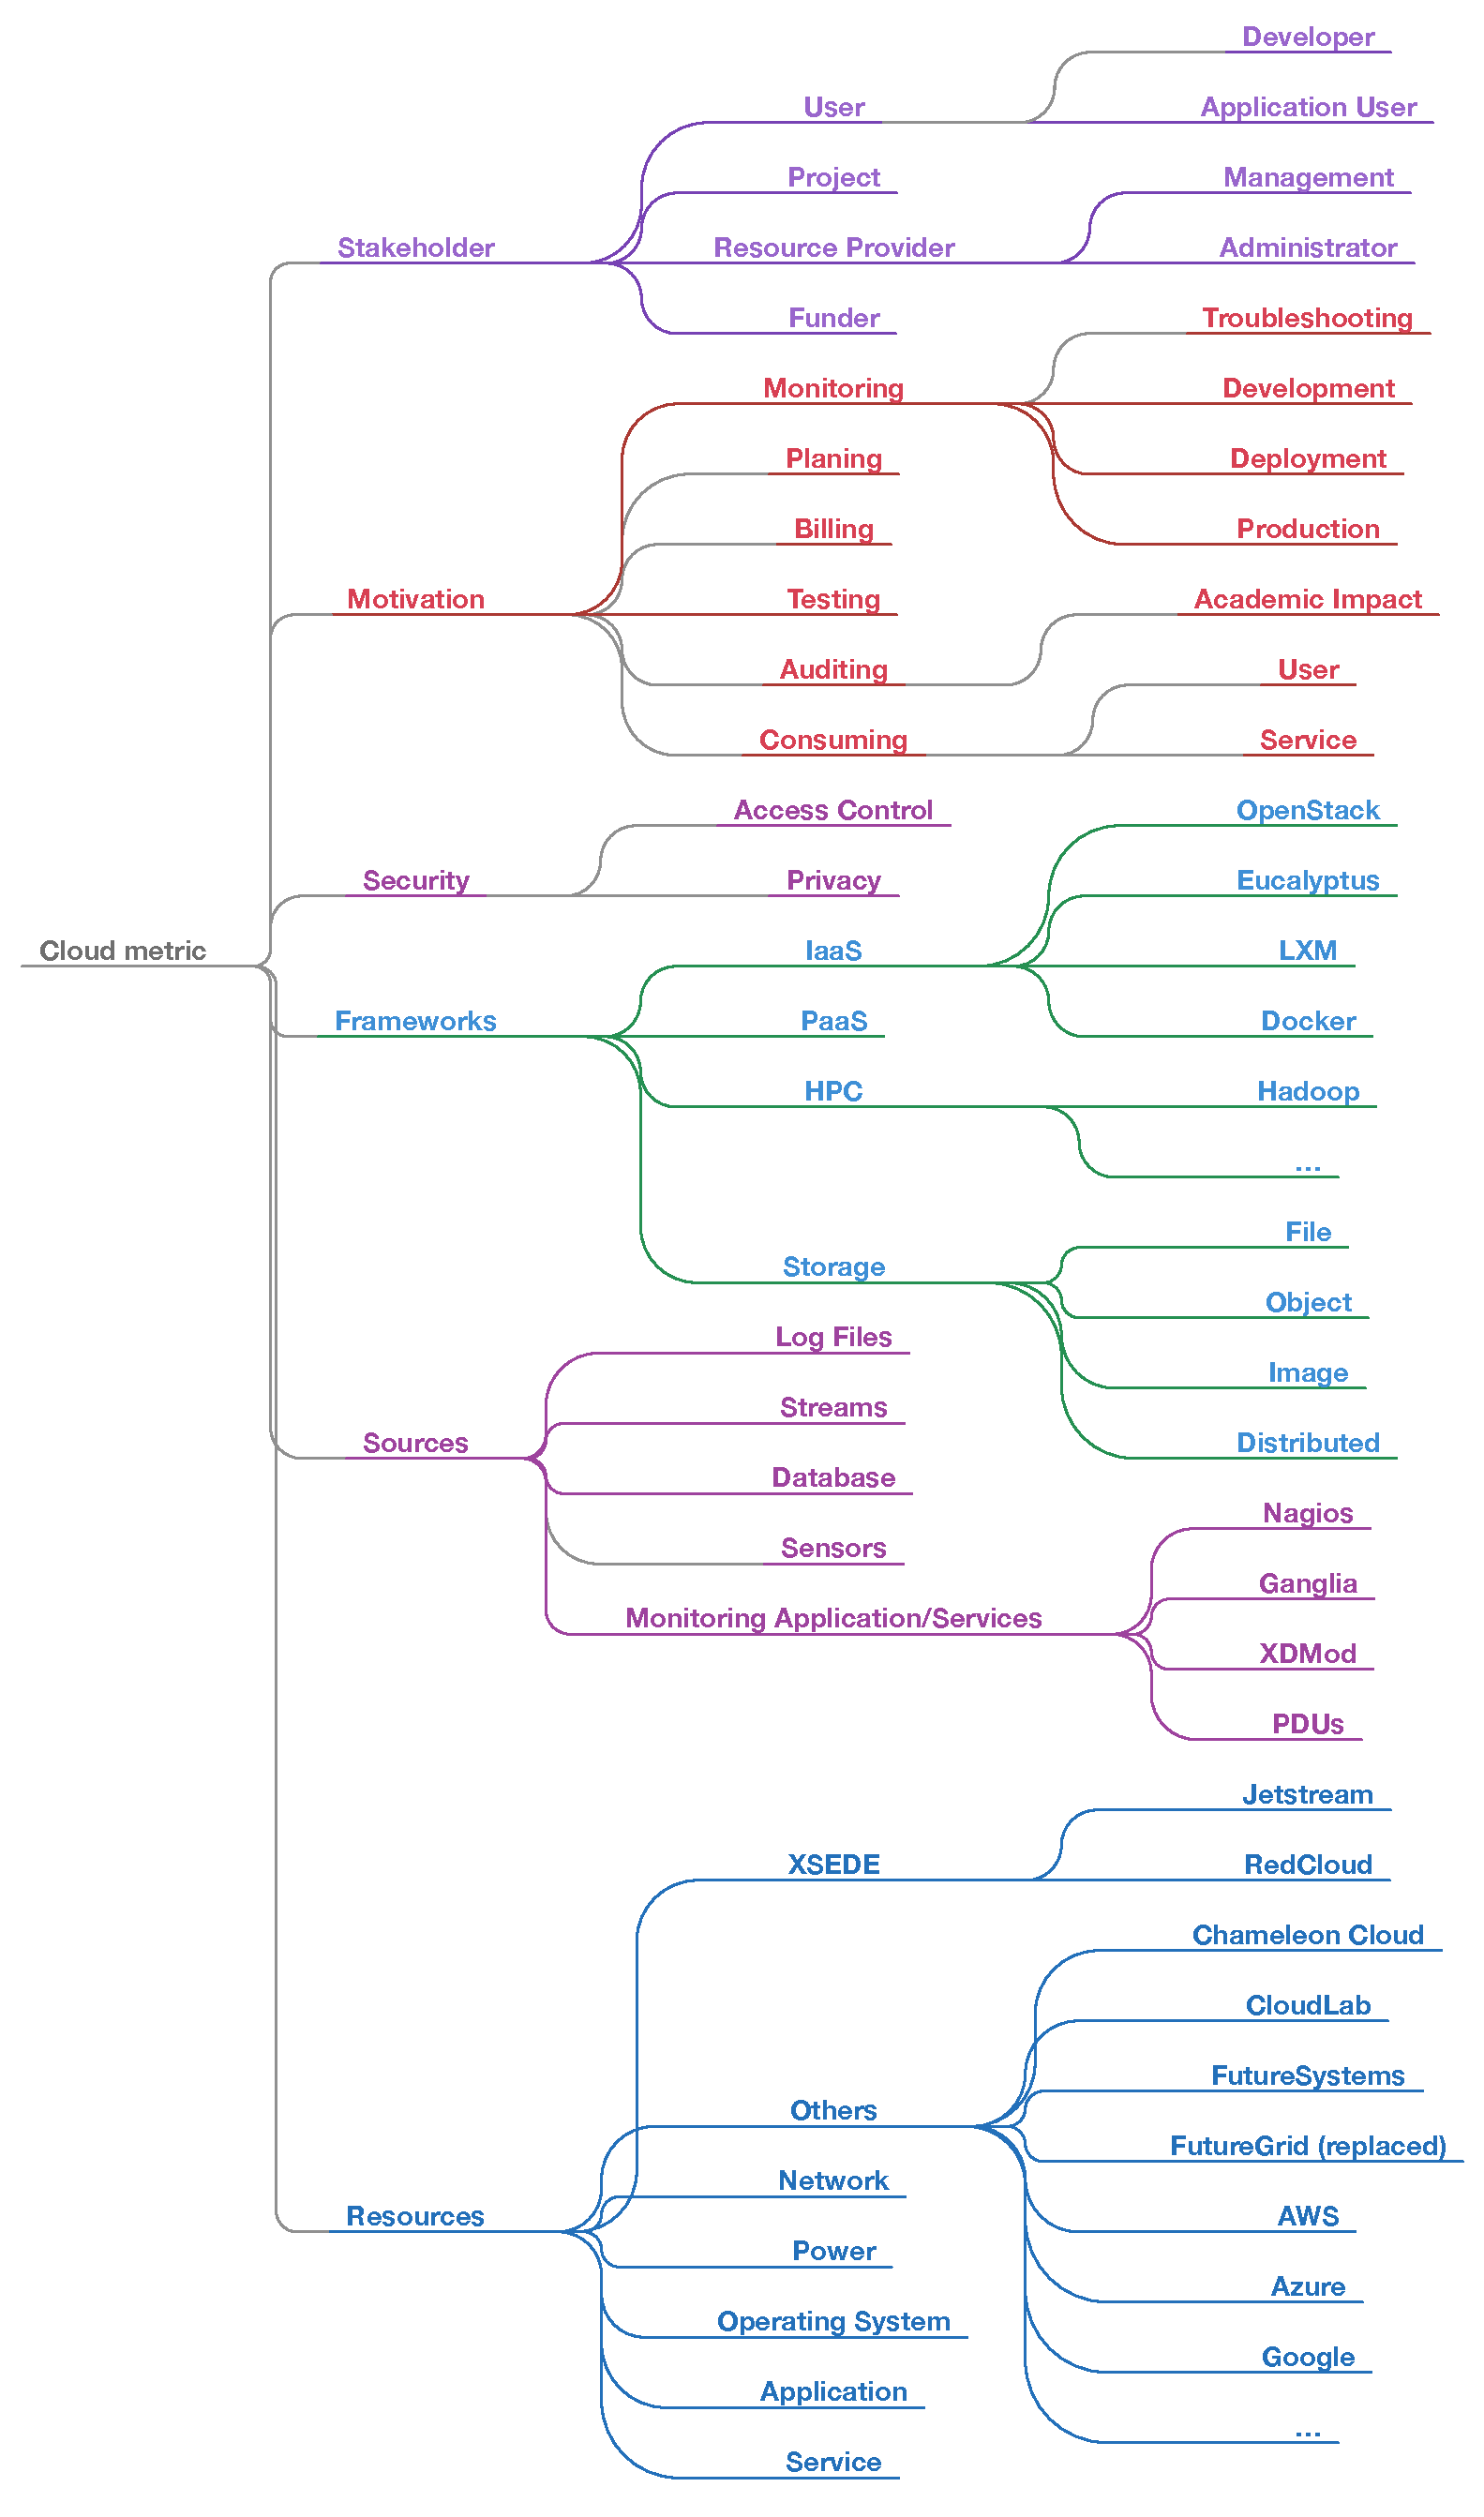
\includegraphics[width=1.0\columnwidth]{images/cloudmetric.pdf}}
   \caption{Overview of cloud metric factors}\label{F:taxonomy-1} 
%\end{figure} 

%\begin{figure}[htb]
\begin{center}
\begin{tiny}
\begin{fTREE}{0.9in}  \Tree
     [. Stakeholder
        [. Funder [.User ]
	   	  [.Project ]
		  [.{University} 
			[. {Production IT} ]
			[. {Research IT} ]
		  	[. {Research Institution} ]
		  ]
		  [.Agency 
			[. {NSF - Directorate} ]
			[. {DOE} ]
			[. {NIH} ]
                  ]
        ] 		
        [.{Resource Provider}
	   	  [.Management ]
		  [.Administrators ]
	]
        [.{Sponsored Project} 
                [. {Principal Investigator} ]
                [. {Project Manager} ]
                [. {Project Members} ]
        ]
	[.{Sponsored User} ]
    [.{Consuming Services } ]
   ]
\end{fTREE}
\end{tiny}
\end{center}
\vspace{-12pt}
\caption{Cloud metric stakeholders}
\label{F:stakeholder}
\end{figure}



\subsection{Stakeholder}

An academic cloud will have a wide variety of stakeholders with potentially very specific and complex needs in regards to metrics. These stakeholders include (a) application developers and users, (b) projects in which multiple users contribute (c) the resource provider including administrators and management including the director. Furthermore, we identify the funder of the cloud as an important stakeholder as he may have needs for specific metrics that are typically not relevant to users or administrators of the cloud but have profound impact on the goal of justifying and delivering funding of resources and projects. To give an example of the wide variety of metrics needed we like to raise awareness of that although management is interested in operational 24/7 operation of the system and statistics associated with it, concrete metrics and monitoring infrastructure as needed by the administrators to detect operational failures are typically not part of the needed metrics for a center director. On the other hand metrics to identify ethnicity and classification into scientific disciplines are of great value for center directors and funders, while they play no importance to the operational metrics to keep the system running. One of the stakeholders also includes consuming services that are authorized to use the metric information to improve via the service offered the underlying resource and service infrastructure. Such consuming services often act in behalf of the previous stakeholders. We list the main stakeholders in Figure \ref{F:stakeholder}.
 

\subsection{Access and Presentation}

Due to this wide range of users that are in the need of metrics it is important to support also the needs of accessing the metrics accordingly. This includes portal information for management and high level users, but also access as part of scripts, APIs and REST services (see Figure \ref{F:access}).

\begin{figure}[htb]
\begin{center}
\begin{tiny}
\begin{fTREE}{.9in}  \Tree
     [. Access
        [. API ]
	[. REST ]
	[. Command 
            [. line ]
            [. shell ]
        ]
	[. Portal ]
   ]
\end{fTREE}
\end{tiny}
\end{center}
\vspace{-12pt}
\caption{Cloud metric access}
\label{F:access}
\end{figure}

Related to the access is naturally how the final information is presented as indicated in in Figure \ref{F:type}.

%%%%%%%%%%%%%%%%%%%%%%%%%%%%%%%%%%%%%%%%%%%%%%%%%%%%%%%%%
\subsection{Information Presentation Type}
%%%%%%%%%%%%%%%%%%%%%%%%%%%%%%%%%%%%%%%%%%%%%%%%%%%%%%%%%
It is clear that the data needs to be presented in a consumable fashion to the stakeholders. In particular we are interested in automatically generating periodic reports on a monthly or quarterly basis, but also support the creation of ad-hoc reports that show the actual current state (see Figure~\ref{F:type}). This is facilitated by interactive services that not only allow the exposure through human readable reports, but also through service consumable reports while using data formats such as XML, YAML, or JSON. In some cases it may also be important to expose the original data. 



\begin{figure}[htb]
\begin{center}
\begin{tiny}
\begin{fTREE}{.95in}  \Tree
[. Type
        [. {\iFILES ~ Report} 
     		[. {Chart} 
           		[. {\iCHART ~ Pie} ]
            	[. {\iTABLE ~ Table} ]
            	[. {\iSTAT ~ Line} ]
            	[. {\iCHARTS ~ Histogram} ]
        ]
	]
      [. {\iCLUSTER ~ Mashup} 
            [. Format
       		[. {XML} ]
        		[. {YAML} ]
        		[. {JSON} ]
			[. {original} ]
		]
         ]
        [. {\iDISPLAY ~ Interactive} 
		[. {see Report \& Mashup} ]
	  ]
     ] 
\end{fTREE}
\end{tiny}
\end{center}
\vspace{-12pt}
\caption{Cloud metric presentation types}
\label{F:type}
 \end{figure}

\subsection{Motivation}

Obviously one very important factor for a cloud metric is the motivation and purpose for it. This factor may significantly impact the purpose and design of the metrics framework we need in order to support the stakeholders. We distinguish the following motivational factors:


\begin{description}
\setlength\itemsep{-2pt}

\item[\it Monitoring.] Monitoring is an important aspect for administrators but also for users. The purpose of metrics associated to monitoring allows us to observe the current system and make decisions based upon it. Naturally, this could also be services that act in behalf of the user or administrator. A center director may be interested in the high level aspects of monitoring as to be informed about specific catastrophic service events, while an administrator is interested in more detailed monitoring aspects that alert even on conditions that could lead to issues. Examples for monitoring includes measuring resource utilization in real time or over a period of time.  Monitoring is potentially important on all layers of the Cloud infrastructure from bare metal, to IaaS, PaaS, and SaaS.

\item[\it Planning.] Planning is needed to assist in setting goals and developing strategies. This includes metrics about utilization of the resources, satisfaction by the users and other more general aspects. As academic resources are often funded by government organizations such as NSF, specific metrics that answer to broader impacts need to be addressed. An essential ingredient of planning is the ability to include performance monitoring on the cloud while exposing sophisticated metrics.  This will enable the planning of efficient resource utilization from a small instance to a large virtual cluster on the cloud, performance management and monitoring are necessary for performance analysis.

\item[\it Billing.] As academic clouds are provided free to the academic user community upon peer reviewed projects, it is also important to avoid situations that either over utilize the resource or adversely lead to underutilization. For example in absence of billing against real monetary values, we observed that many users ignore the cost that is involved by running an actual VM. They keep on running it despite the fact that they may not need it anymore and no panelity is provided for keeping instances running. Hence, it is important to communicate to the users the potential estimated cost to them in order to educate them towards deleting or suspending unused resources. However, at the same time it must be assured that large enough experiments can be conducted to further some of the more challenging scientific problems and strike a compromise as part of {\it billing} a project.

\item[\it Testing.] As cloud environments and they usage in applications may be complex (at times more complex that their HPC counter parts) it is important that metrics be provided that support the testing of the functionality, the performance, and the scalability. Ideally these metrics should be available as part of automatic testing services that however may be customized for a particular application.

\item[\it Consuming.] Many metrics will assist the users and services to consume the cloud services efficiently. They will provide information in optimizing resource use and distribution amongst them. They will also alert towards limitations of the underlying systems and provide insight on where application limitations my hinder adoption. A specific case is the creation of user motivated benchmarks that through their metrics can inform users about which cloud setup is particularly beneficial.

\item[\it Auditing.] Metrics for auditing support the process to evaluate the clouds design and effectiveness. This includes security, deployment processes, development processes and governance and oversight processes.  It includes finding a proof and a trait of actions a user made while resources are being used. Observing a user's, or service's behavior should be performed by logging events and detailed information is necessary to track back any issues on a system.  An important aspect or a comprehensive auditing process is that that it is conducted by an independent and unbiased observer. Auditing should not be confused with monitoring the system in real time.

\end{description}


\subsection{Security}

Due to targeting different user communities it is obvious that some metrics may not be exposed to all of its academic users and need to be placed under access control. Furthermore, users that consume cloud resources may have the desire that their information is private and may not be shared with other users. However, although it is possible to provide access and privacy controls we have see in government agency sponsored research environments (such as NSF) a general consensus of transparency mandated by the funding agency. A good example here is XSEDE that provides a great deal of information to its users in a transparent fashion. When looking at a metric framework for clouds we need to consider the possibility to restrict certain information through access control policies that regulate privacy concerns. Such policies need to include role-based restrictions of stakeholders and metrics to be accessed by them. It is clear that many metrics that are actually collected may assist in making the underlying services and resources more secure. Hence metrics in regards to intrusion detection, system flaws, identity management and application security are of special importance. Collecting this information over a longer period of time can provide a great deal of information if specific areas in regards to security need to be addressed or improved. Part of this information may need to be protected. We summarize the different factors in Figure \ref{F:security}.



\begin{figure}[htb]
\begin{center}
\begin{tiny}
\begin{fTREE}{.9in}  \Tree
     [. Security
        [. {Access}
           [. {Access control} ]
	     [. Privacy ]
	     [. Encryption ] 
	     [. Obfuscation ]
        ]
        [. {Service Support}
		[. {Intrusion detection} ]
		[. {System flaws} ]
		[. {Identity management} ]
		[. {Application security} ]
	]
   ]
\end{fTREE}
\end{tiny}
\end{center}
\vspace{-12pt}
\caption{Cloud metric security factors.}
\label{F:security}
 \end{figure}



\subsection{Service Frameworks}

As already pointed out in the introduction, it is important to not isolate the cloud metrics and limit the metrics to IaaS frameworks. This includes the integration of high performance computing resources and services (HPC), storage resources and services, infrastructure as a service based resources build from either OpenStack, VM Ware, or Nimbus, as well as various platform as a service environments that enable academic users to focus on the platform regardless of which underlying resource framework is chosen.  Furthermore it may be important to consider extending the cloud metrics framework to public clouds such as AWS, Azure, Google and others as this may be an integral part of the strategy to offer cloud services to academic user communities. Restrictions posed by some of these frameworks such as the lack of groups in the Nimbus framework make it problematic to meet the demands from well established accounting metrics as provided by for example XSEDE. Thus if an IaaS framework such as Nimbus is to be deployed meaningful in academic project based resource framework appropriate changes may need to be conducted that are readily offered by for example OpenStack and Eucalyptus. Hence we can see that a lack of features (despite offering others such as auto-scaling) may contradict established policies and mechanism introduced by previous efforts. In such cases it needs to be evaluated if such services should be offered. In case of Nimbus the FutureGrid team at IU developed a process to associate user projects based on assignment to project groups to fulfill our internal policies.  We summarize the different factors regarding service frameworks in Figure \ref{F:frameworks}.



\begin{figure}[htb]
\begin{center}
\begin{tiny}
\begin{fTREE}{.9in}  \Tree
     [. Frameworks
        [. {IaaS}
           [. {Nimbus } ]
	      [. OpenStack ]
	      [. Eucalyptus ] 
	      [. Azure ]
		[. Google ]
        ]
        [. {PaaS} ]
        [. {HPC} ]
	  [. {Storage} ]
]
\end{fTREE}
\end{tiny}
\end{center}
\vspace{-12pt}
\caption{Cloud metric applied to service frameworks.}
\label{F:frameworks}
 \end{figure}


\subsection{Resources}\label {S:resources}

Metrics that are implicitly provided by various cloud providers are important for gaining a complete picture of a particular project. This may include the following

\begin{description}
\setlength\itemsep{-2pt}

\item[\it Commercial public clouds.] These are clouds that are offered commercially or for free for a limited time to academic research and education users. While metrics for individuals that use such services for free may initially not be of importance, it becomes essential if at one point actual money is paid to provide this service to the academic user, project, or institute. Important may not only the amount of money paid, but to justify the expense through academic and scientific impact \cite{las2015cluster,las2015xsede} that is derived by such efforts.

\item[\it Academic public clouds.] Recently NSF has provided a significant amount of funding to cloud offerings for the academic community \cite{??chameleon,www-cloudlab,??jetstreem}. In order to justify their funding and to contrast it to commercial public cloud offerings metrics and evaluation criteria need to be developed that allow meaningful comparisions.

\item[\it Academic private clouds.] Many universities have started to offer private clouds to their research community. This includes not only the use of academic efforts, but as previously stated also of production clouds to support the internal IT infrastructure as part of a universities management IT infrastructure. While in the IT department operational cost and privacy are potentially dominating the metrics, in academic clouds the use in projects and their outcome metrics need to be integrated. This reflects similar metrics that we find while using commercial and academic public clouds.

\end{description}

We summarize the different factors regarding resource types in Figure \ref{F:frameworks}.



\begin{figure}[htb]
\begin{center}
\begin{tiny}
\begin{fTREE}{1.2in}  \Tree
     [. Resource
        [. {Commercial Public Clouds} 
		[. {AWS \cite{www-aws}} ]
		[. {Azure \cite{??}} ]
        ]
        [. {Academic Public Clouds} 
	      [. {FutureSystems \cite{??}} ] 
            [. {Jetstream \cite{??}} ]
	      [. {Chameleon Cloud \cite{??}} ]
	      [. {CloudLab \cite{www-cloudlab}} ] 
	  ]
        [. {Academic Private Clouds} 
    		[. {UB Eucalyptus \cite{www-eucalyptus} } ]
	  ]
]
\end{fTREE}
\end{tiny}
\end{center}
\vspace{-12pt}
\caption{Cloud metric applied to service frameworks.}
\label{F:frameworks}
 \end{figure}


Examples for publicly funded clouds include XSEDE\cite{??} while offering HPC services to its users\footnote{We argue that XSEDE in general can be viewed as a resource that offers HPC as a service to its user community.}, Chameleon Cloud \cite{??}, CloudLab \cite{??}, as IaaS based clouds and network experiment infrastructure, and Jetstream \cite{??} as Iaas and PaaS supporting cloud. These organization provide resources and services to many users. Other efforts such as FutureSystems \cite{??} offer large resources to a selected small set of users thus increasing the availability of a scalable environment.

Additionally the following cloud related resources offered to academic users will have a potential impact on the definition of Metrics:

\begin{description}
\setlength\itemsep{-2pt}

\item[\it MRIs.] According to the NSF web pages, the `Major Research Instrumentation Program (MRI) ~\cite{nsf-mri} catalyzes new knowledge and discoveries by empowering the Nation's scientists and engineers with state-of-the-art research instrumentation. The MRI Program enables research-intensive learning environments that promote the development of a diverse workforce and next generation instrumentation, as well as facilitates academic and private sector partnerships.'' Some of the MRI funding supports significant computational resources offered to a particular user community. In such cases it would be beneficial if the metrics and services introduced here can be reused by such efforts and adapted accordingly.

\hyungro{mine cloud related activities from NSF. \url{http://www.nsf.gov/awardsearch/advancedSearchResult?ProgEleCode=1189&BooleanElement=ANY&BooleanRef=ANY&ActiveAwards=true&}}

\item[\it Networks.] With the advent of 100GBEthernet research environments as provided in Jetstream, Chameleon cloud and XSEDE it is essential that network related information be integrated into an overarching metric framework. This includes not only details of the overall use of the network, but the specific information which projects, or even which applications are using it. Access control to this information may has to be investigated in order not to expose exploitable information to the community. Typically we find that this information is not yet sufficiently communicated in a transparent way to the diverse research and education community.

\item[\it Storage.] Obviously many cloud applications in the big data area require large amount of storage either as files, databases, or object stores. Metrics must be available to the users and the providers in order to assess needs and availability. Storage has traditionally been an issue in academic environments.

\item[\it Power.] A significant cost in operating an academic cloud is power consumption. It is important that the IT departments of the academic cloud providers put efforts in place that power usage is transparently exposed so that associations between power and services offered can be achieved. This goes beyond the measurement of power consumption within servers, but must include a more generalized approach while integrating PDU information, air conditioning and other energy driving factors while integrating and correlate them with other available metrics. However, typically such information is often isolated and potentially not available to the academic user community without a significant effort. Future designs of academic datacenter should keep in mind that such information ought to be transparently provided to the researchers or retrofitted accordingly. Production academic IT departments must project a way forward that such information is exposed transparently to the researchers. Purchase of such equipment may need to provide appropriate safegurads and the ability to share the data with the researchers in a programmatic fashion.

\item[\it Operating Systems.] Traditionally a large amount of metric information is available as part of the operating system either in virtualized or in bare metal mode. The included services can present a great deal of information to users and to the resource provider. Tools such as Nagios \cite{??} and Ganglia \cite{??} provide the ability to collect and integrate the information sources.

\item[\it Applications.] Many academic users will develop a number of applications on available resources. Metrics that compare efficiency and effective use of such applications will be important as to evaluate prudent use of the resources. For example in some cases it may be essential to measure the performance impact of using cloud vs. HPC resources. In other cases it may be more important to focus on manpower consumed to develop applications on more complex environments. Supporting performance APIs and libraries may aide in the development of metrics and their associated services such as the use of PAPI \cite{papi2014,papi-web,JohnNelsonAnalyzingPAPI}

\item[\it Services.] In addition to applications we also are in the need of metrics provided by services offered to the community.

\end{description}

\subsection{Information Sources}

A comprehensive metrics framework consists of a data mashup of various sources of information. It will not be sufficient to just present a heterogeneous set of metrics to the users, but it will be desirable to integrate several into an easy to use framework. This has been effectively demonstrated by XDMod for HPC \cite{las14cloudmeshmultiple,las14Impact,las12xdmod-kernel}. This was possible due to a sustained effort within the project to provide such integrated metrics. In the cloud IaaS area the FutureGrid project has pioneered such an integrated framework that combined multiple sources into an easy to use report generation framework \cite{LeeFGresource}. It was operational for a number of years and is still actively used by the FutureSystems project. In fact there may be an implicit advantage that the same metrics that were collected by employed in activities such as CloudLab, Chameleon and Cloudmesh. We observe however that many metrics in regards to project information are not implementable due to a lack of information gathered at the time the project is proposed. This also includes information that is not yet collected as part of the XSEDE XRAC process. We found that a more sophisticated information gathering allowed us to greatly streamline our efforts in FutureGrid (for example the dominance of OpenStack as the IaaS framework of choice at the end of FutureGrids funding cycle)

\begin{comment}
\begin{figure*}[htb] 
  \centering 
    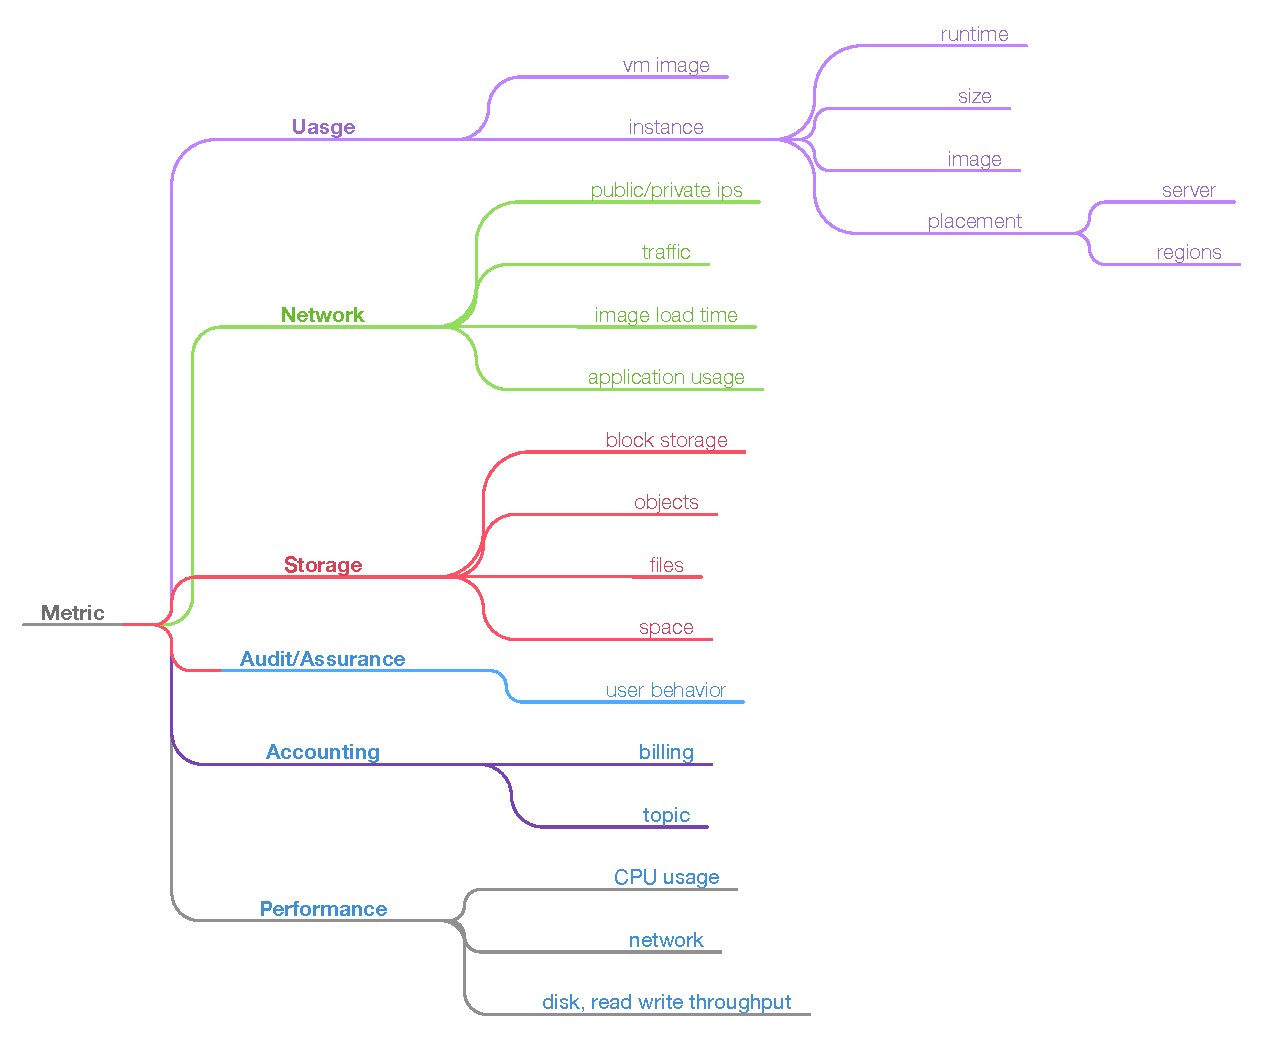
\includegraphics[width=0.6\textwidth]{images/cloudmetric-2.pdf} 
  \caption{Overview of CloudMetrics.}\label{F:taxonomy-2} 
\end{figure*} 
\end{comment}



\begin{table*}[P]
\caption{Selected scientific impact metrics.}
\begin{scriptsize}
\label{T:SIMmetrics}
\bigskip
\begin{center}
\begin{tabular}{p{0.19\textwidth}p{0.38\textwidth}p{0.38\textwidth}}
\hline
\rowcolor{blue!20}  \bf  Name & \bf Description & \bf Motivation \\
\hline
Publication Count &
Measuring how many publications are attributed as output while using the cloud 
resource &
Measures the general productivity \\
\hline 
Citation Count &
Measuring how many citations has been received as of the measuring time point &
Shows how the output really impacts the scientific community while the 
publications are being cited \\
\hline
H-index (person) \cite{hirsch2005index} &
A person has index $h$ if $h$ of his/her $N_p$ papers have at least h
                   citations each, and the other $(N_p − h)$ papers have
                   no more than $h$ citations each. &
Measures both productivity and the generated impact \\
\hline
G-index (person) \cite{egghe2006theory} &
Given a set of articles ranked in decreasing order of the number of citations that they received, the $g$-index is the (unique) largest number such that the top $g$ articles received (together) at least $g^2$ citations.&
Depends on the full citation count of very highly cited papers\\
\hline
H-index (entity) &
While treating the evaluated entity as if it were a person, using the
h-index that were originally defined for a person &
Measures both productivity and the generated impact \\
\hline
G-index (entity)&
While treating the evaluated entity as if it were a person, using 
g-index that were originally defined for a person &
Measures both productivity and the generated impact \\
\hline
i10-index \cite{www-i10index} &
Number of publications cited as least 10 times &
How many publications have achieved a certain level of impact (based on citation count) \\
\hline
ptrank-citation \cite{las14Impact,las15xsede,las15cluster} &
Percentile rank of citation count among peers &
To compare the studied entity's relative impact with the peers. The peers are identifie as publicatons that were published in same issue of the same journal for a publication that belongs to the studied entity (e.g., a journal, a Field of Science, the whole system, etc.) \\
\hline
\end{tabular}
\end{center}
\end{scriptsize}
\end{table*}


\subsection{Scientific Impact}

Many science and engineering innovations and discoveries are increasingly dependent on access to high performance computing resources \cite{las14Impact,las15xsede,las15cluster}. For many researchers, this demand is met by clouds and other large-scale compute resources that cannot typically be supported by any single research group. Accordingly, dedicated large-scale computing facilities play an important role in scientific research, in which resources are shared among groups of researchers, while the facilities themselves are managed by dedicated staff.  Thus, justification for their use is warranted and questions regarding the scientific impact of these resources naturally arise. Hence, it is important to not only introduce metrics measuring the actual usage, but also the impact based on for example the scientific publications that are produced by such resources. We have developed a sophisticated metric framework that delivers such impact metrics for XSEDE, NCAR, and Blue Waters \cite{las14Impact,las15xsede,las15cluster}. It is most natural that this be extended to any cloud resource. However, the framework is general enough that it could apply to any resource framework and interested resource providers can contact the corresponding author\footnote{send email to {\textit laszewski@gmail.com}} for more information. Table \ref{T:SIMmetrics} lists the general metrics related to the impact of scientific works.

While evaluating a research computing facility (in this context, a cloud resource provider) based on how the accounting and auditing framework is setup, as well as the mechanism of gathering publications as output of using the cloud. A suite of different metrics has been useful and a subset of the most useful once are listed in Table \ref{T:SIMmetrics}.  Our scientific impact process can be  applied, if we have user and group/project units in the accounting system, and the publications are gathered and vetted also with user/group/project information, we could derive the same metrics for each user, group/project, and compare their performance.  Consequently, these metrics can be calculated for a cloud resource provider as a whole entity, and the same metrics could be compared among different cloud resource provider. Based on other related data, e.g. the resource had been consumed, we could derive and compare the same metrics but in a normalized fashion - Publication count and/or citation count per CpuHours as an example. An important distinction of our work includes a peer comparison metric that we term {\it ptrank-citation} and is explained in detail in \cite{las14Impact,las15xsede,las15cluster}. Such comparison is possible based on or data mashup with millions of references, while at the same time focusing on the comparison of publications related to our resource to be analyzed.


\afterpage{\begin{table*}[P]
\caption{User related metrics.}
\label{T:metrics-bigtable}
\bigskip
\begin{scriptsize}
\begin{center}
\begin{tabular}{lp{0.1\textwidth}p{0.4\textwidth}p{0.4\textwidth}}
\hline
\rowcolor{blue!20} \bf ID & \bf Name & \bf Description & \bf Motivation \\
\hline
UC.1&
User Count & 
 counts the active users for the cloud &
User count is important for measuring the popularity of the cloud \\
\hline
UC.2&
Major Users &
heavy users in terms of consuming resources e.g. top 10 users &
Top 10 Users is important to see who has the most impact on the shared resources \\
\hline
UC.3 &
User Type &
a user type defined in an account system with a percentage of
the total numbers. e.g. a project leader, an instructor, or a students. & 
User Type is important to see a proportion of users.  \\
\hline
UC.4 &
Repeat User&
the number of users who actively using services for a certain period.  e.g. last 3/6/9 month: 16/32/24 &
Repeat User is important for measuring user activity for a certain period \\
\hline
UD.1 &
Tenant Distribution&
a proper balancing of resources per tenant. &
Tenant Distribution is important to see users spread evenly across compute nodes \\
\hline
\end{tabular}
\end{center}
\end{scriptsize}
\end{table*}


\begin{table*}[P]
\caption{Virtual machine metrics.}
\begin{scriptsize}
\label{T:metrics}
\bigskip
\begin{center}
\begin{tabular}{lp{0.1\textwidth}p{0.4\textwidth}p{0.4\textwidth}}
\hline
\rowcolor{blue!20} \bf ID & \bf Name & \bf Description & \bf Motivation \\
\hline 
VC.1&
VM Count & 
 counts the launched VM instances on the cloud &
VM Count is important for measuring the volume of requested instances \\
\hline
VC.2&
VM Count by Project, Leader, or Institution &
share of resource by group metrics such as project, leader or institution &
Group usage is important for measuring group usage \\
\hline
VC.3 &
Current running VMs or accessed users &
instant usage data to see current status &
real time usage is important for checking peak or detecting unusual usage \\
\hline
VCT.1 &
VM Creation Time &
the latency of creating a new instance to ensure fast creation &
VM Create Time is important for measuring the latency \\
\hline
VRS.1&
VM Runtime Sum&
the total amount of runtime for launched instances &
runtime by hour is important for measuring actual runtime of instances \\
\hline
VCC.1 &
vCPU Usage &
the number of vCPU cores allocated to instances &
vCPU Usage is important for measuring system resource used \\
\hline
VM.1 &
Memory Usage &
the size of memories allocated to instances &
Memory Usage is important for measuring system resource used \\
\hline
\end{tabular}
\end{center}
\end{scriptsize}
\end{table*}

\begin{table*}[P]
\caption{Image related metrics}
\begin{scriptsize}
\label{T:metrics}
\bigskip
\begin{center}
\begin{tabular}{lp{0.1\textwidth}p{0.4\textwidth}p{0.4\textwidth}}
\hline
\rowcolor{blue!20} \bf ID & \bf Name & \bf Description & \bf Motivation \\
\hline 
IC.1 &
Image Type &
an image type registered in the cloud platforms with a
percentage of the total number. e.g. ubuntu14.04, centOS 7, or Fedora 22 & 
Image Type is important to see a proportion of images. \\
\hline
\end{tabular}
\end{center}
\end{scriptsize}
\end{table*}

\begin{table*}[P]
\caption{Flavor related metrics.}
\begin{scriptsize}
\label{T:metrics}
\bigskip
\begin{center}
\begin{tabular}{lp{0.1\textwidth}p{0.4\textwidth}p{0.4\textwidth}}
\hline
\rowcolor{blue!20} \bf ID & \bf Name & \bf Description & \bf Motivation \\
\hline 
FC.1 &
Flavor Type &
an flavor (instance) type registered in the cloud platforms with a
percentage of the total number. e.g. m1.small, m1.medium, or m1.xlarge & 
Flavor Type is important to see a proportion of instance types. \\
~\\
\hline
\end{tabular}
\end{center}
\end{scriptsize}
\end{table*}

\begin{table*}[P]
\caption{Storage related metrics}
\begin{scriptsize}
\label{T:metrics}
\bigskip
\begin{center}
\begin{tabular}{lp{0.1\textwidth}p{0.4\textwidth}p{0.4\textwidth}}
\hline
\rowcolor{blue!20}   \bf ID & \bf Name & \bf Description & \bf Motivation \\
\hline  
DU.1 &
Disk Usage &
the size of Disks allocated to instances &
Disk Usage is important for measuring system resource used \\
\hline
DU.2 &
Object Usage &
the size of Object Storage allocated to instances &
Object Usage is important for measuring system resource used \\
\hline
DU.3 &
Block Usage &
the size of storage blocks mounted to instances &
Block Usage is important for measuring system resource used \\
\hline
\end{tabular}
\end{center}
\end{scriptsize}
\end{table*}

\begin{table*}[P]
\caption{Server related metrics}
\begin{scriptsize}
\label{T:metrics}
\bigskip
\begin{center}
\begin{tabular}{lp{0.1\textwidth}p{0.4\textwidth}p{0.4\textwidth}}
\hline
\rowcolor{blue!20}   \bf ID & \bf Name & \bf Description & \bf Motivation \\
\hline
SC.1 & 
Node Distribution & 
a physical node distribution. & 
Node Distribution is important for load balancing. \\
\hline
SP.1 &
Power Consumption&
the amount of energy used in the cloud platform  &
Electricity is important for measuring actual cost by Kilo Watt per hour (KWh) \\
\hline
SA.1 &
Availability&
a percentage rate of available resources to accept a new request &
Availability is important to provide cloud resources continuously \\
\hline
SSC.1 &
Scalability \& Capacity&
an actual limit of a service or physical system in the cloud &
Scalability and Capacity are important to measure IaaS performance \\
\hline
ST.1 &
Throughput &
the performance of cloud services by measuring completed tasks, i.e. PaaS &
Throughput is important for measuring service performance e.g. PaaS \\
\hline
SCS.1 &
CPU Speed (system performance)&
the performance of cloud resources by clock speed of a processor &
CPU Clock speed is important to understand an actual speed of CPUs over different cloud platforms \\
\hline
SMS.1 &
Memory Speed (system performance)&
the performance of cloud resources by clock speed of a memory &
Memory Clock speed is important to understand an actual speed of memories over different cloud platforms \\
\hline
SDS.1 &
Disk Speed (system performance)&
the performance of cloud resources by read/write speed of a disk including SSD &
Disk speed is important to understand an actual speed of disks over
                                                                                 different disk types \\
\hline
\end{tabular}
\end{center}
\end{scriptsize}
\end{table*}

\begin{table*}[P]
\caption{Network related metrics.}
\begin{scriptsize}
\label{T:metrics}
\bigskip
\begin{center}
\begin{tabular}{lp{0.1\textwidth}p{0.4\textwidth}p{0.4\textwidth}}
\hline
\rowcolor{blue!20} \bf ID & \bf Name & \bf Description & \bf Motivation \\
\hline
NL.1 &
Latency &
a network and application performance &
Latency is important with acceptable and strict latency expectation \\
\hline
NT.2 &
Network Throughput&
the actual amount of data delivered successfully &
Network thoughput is important for measuring network performance \\
\hline
NP.3 &
PublicIP Count &
availability of public IP addresses. &
PublicIP Count is important for the number of available and free IP addresses. \\
\hline
NP.3 &
PriveIP Count &
availability of private IP addresses. &
PrivateIP Count is important for the number of available and free IP addresses. \\
\hline
\end{tabular}
\end{center}
\end{scriptsize}
\end{table*}

\begin{table*}[P]
\caption{Project related metrics.}
\begin{scriptsize}
\label{T:metrics}
\bigskip
\begin{center}
\begin{tabular}{lp{0.1\textwidth}p{0.4\textwidth}p{0.4\textwidth}}
\hline
\rowcolor{blue!20} \bf ID & \bf Name & \bf Description & \bf Motivation \\
\hline 
PC.1 & Number of projects & 
the cumulative number of projects & 
Project Count is important for measuring growth of use, time periods:
                                    daily, \\
\hline
PC.2 & Number of projects by discipline & 
the cumulative number of projects by discipline &
Project Count by discipline is important to understand the growth of use by
field of knowledge.  Time periods: daily, monthly, quarterly, yearly \\
\hline
PC.3 & Number of projects by organization & 
the cumulative number of projects by organization &
Project Count by organization is important to understand the growth of use by
institution. Time periods: daily, monthly, qaurterly, yearly \\
\hline
PC.4 & Technology in Use & 
the percentage of technologies and software packages in use & 
Technology in use is important to improve application-based services
                                                              in the \\
\hline
PC.5 & Desired Technology &  
the percentage of technologies and software packages preferred to use &
Preferred Technology is important to understand the needs of software packages
in the cloud \\
\hline
\end{tabular}
\end{center}
\end{scriptsize}
\end{table*}

\begin{table*}[P]
\caption{Region related metrics.}
\begin{scriptsize}
\label{T:metrics}
\bigskip
\begin{center}
\begin{tabular}{lp{0.1\textwidth}p{0.4\textwidth}p{0.4\textwidth}}
\hline
RC.1 & 
Location & 
a geographical location of a user. & 
Location is important for resource availability to different regions. \\
\end{tabular}
\end{center}
\end{scriptsize}
\end{table*}


\clearpage}

%%%%%%%%%%%%%%%%%%%%%%%%%%%%%%%%%%%%%%%%%%%%%%%%%%%%%%%%%%%%%%%%%%%%%%
\section{CLOUD METRICS} \label{S:metrics}
%%%%%%%%%%%%%%%%%%%%%%%%%%%%%%%%%%%%%%%%%%%%%%%%%%%%%%%%%%%%%%%%%%%%%%



In this section we will introduce several important examples for cloud metrics that will be important for academic cloud providers.  Several metrics that we define here are are derived from experience with FutureGrid and FutureSystems. Several dimensions  are influencing the  the metrics (see Figure \ref{F:metric-dimesnion} ) including the time period on which the metric is applied and the value representation.

\begin{figure}[htb] 
  \centering 
    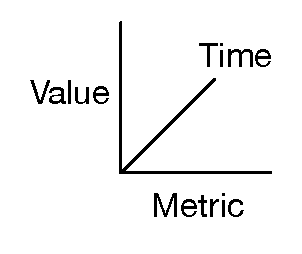
\includegraphics[width=.3\columnwidth]{images/metric-dimension.pdf} 
  \caption{Metric dimensions}\label{F:metric-dimesnion} 
\end{figure} 


\subsection{Time Period}

The time dimension is an importnat dimension of any metrics framework. This includes the following:


\begin{description}
\setlength\itemsep{-2pt}

\item [Period.] Many metrics need to be applied on a flexible period, thus it is important to be able to define the start and end time of a metric to be applied, as well as its periodicity throughout the interval.

\item[Realtime.] Some metrics need to be applied at realtime in order to obtain immideate feedback about the system status

\item[Time to Live.] As some of the metrics may provide a lot of data it is useful to introduce a Time To Live (TTL) that allows metric data to expire if they are no longer needed.
 
\end{description}

\section{Value Representation}

In many cases the data needs to be represented in agglomerated fashion to be easily comprehensible. Typical statistical measurements such as count, sum, mean, median, standard deviation, frequency, distribution, and others. Together these metric properties can be used to provide (a) effective summary reports, (b) periodicity reports (c) real time information. Trough the introduction of stakeholders  some information may be restricted.

Examples of summary reports include walltime of servers used in a cluster as total over a particular time, the VM count, or the user count. Additional factors such as to which project the information is associated is important for project members or for those judging if the resources allocated for a project are justified. Center directors may need to report to their organization which scientific discipline have used the resource. These are just a very small but quite useful set of metrics that have had practical impact in existing academic cloud environments such as FutureGrid and FutureSystems.  For summary reports we also found it useful to overlap multiple metrics into the same chart over a given period. This way we can showcase, contrast or verify trends between different metrics.  To present the information the metrics may need to be able to be conveniently be displayed as charts, as time series data, in tables or json format or through RESTful service.  Properties that are important to consider as part of metrics include scalability, overhead, availability, accuracy, security, agility, and the integration of some of the metrics into autoscaling services.

\subsection{Metrics}

We provide a comprehensive list of useful metrics in Table \ref{T:project} to \ref{T:region}. These tables list a number of important metrics to consider for an academic cloud offering. However, this is just a starting point and additional metrics could useful. Hence we view this list as a starting point and not as a complete closed list of metrics. This also puts an additional requirement on the metrics framework itself. It needs to be easily expandable with new metrics and its data sources.\footnote{If you like to make suggestions of additional metrics, please e-mail to the corresponding author at {\textit laszewski@gmail.com}}

\begin{description}
\setlength\itemsep{-2pt}
\item [Project  management related metrics] (see Table \ref{T:project}). 
\item [User related metrics] (see Table \ref{T:metrics-bigtable}).
\item [Virtual machine metrics] (see Table \ref{T:vm}).
\item [Image related metrics] (see Table \ref{T:image}).
\item [Flavor related metrics] (see Table \ref{T:flavor}).
\item [Storage related metrics] (see Table \ref{T:storage}).
\item [Server related metrics] (see Table \ref{T:server}).
\item [Network related metrics] (see Table \ref{T:network}).
\item [Security related metrics] (see Table \ref{T:security}).
\item [Region related metrics] (see Table \ref{T:region}).
\end{description}


\clearpage

\hyungro{provide simple sceenshots of report figures related to the
  information listed in Fig 1a - 8a or are thes already displayed in
  the last section}

\hyungro{provide a screenshot of the dashboard}

\hyungro{provide a screenshot of a single page of the metric report
  with nice headlines and graphs}

\begin{figure}[h!] 
  \centering 
    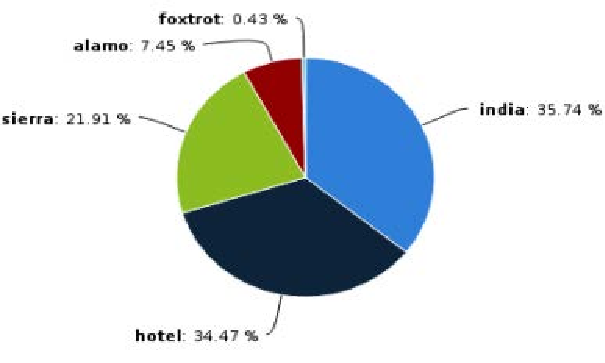
\includegraphics[width=1.0\columnwidth]{images/usercount.pdf} 
  \caption{Active user count by host}\label{F:usercount-1} 
\end{figure} 

\begin{figure}[h!] 
  \centering 
    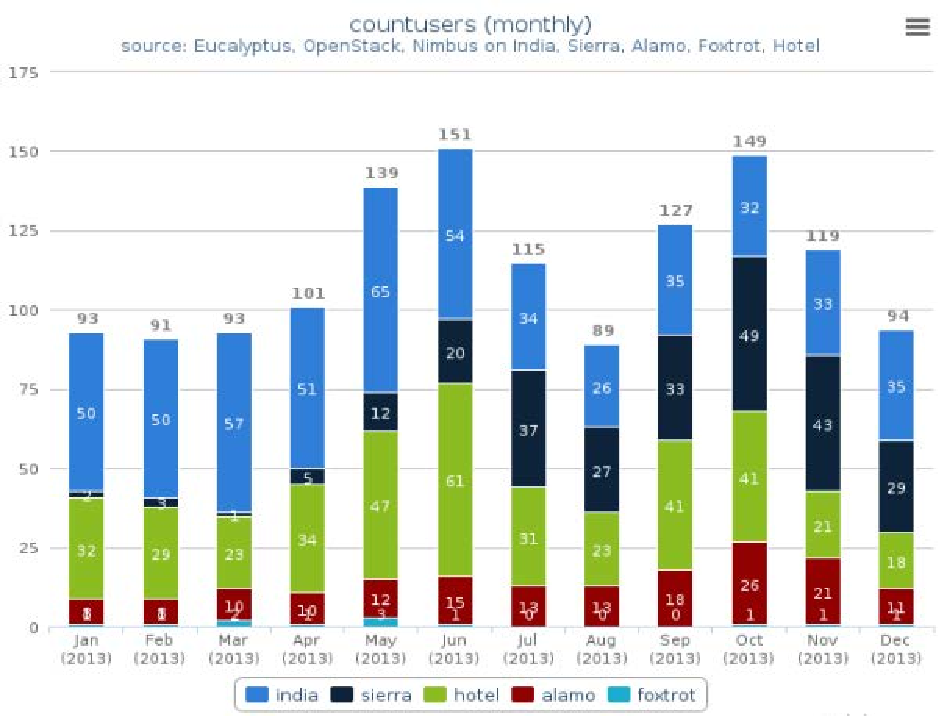
\includegraphics[width=1.0\columnwidth]{images/usercount2.pdf} 
  \caption{Active user count monthly}\label{F:usercount-2} 
\end{figure} 

\begin{figure}[h!] 
  \centering 
    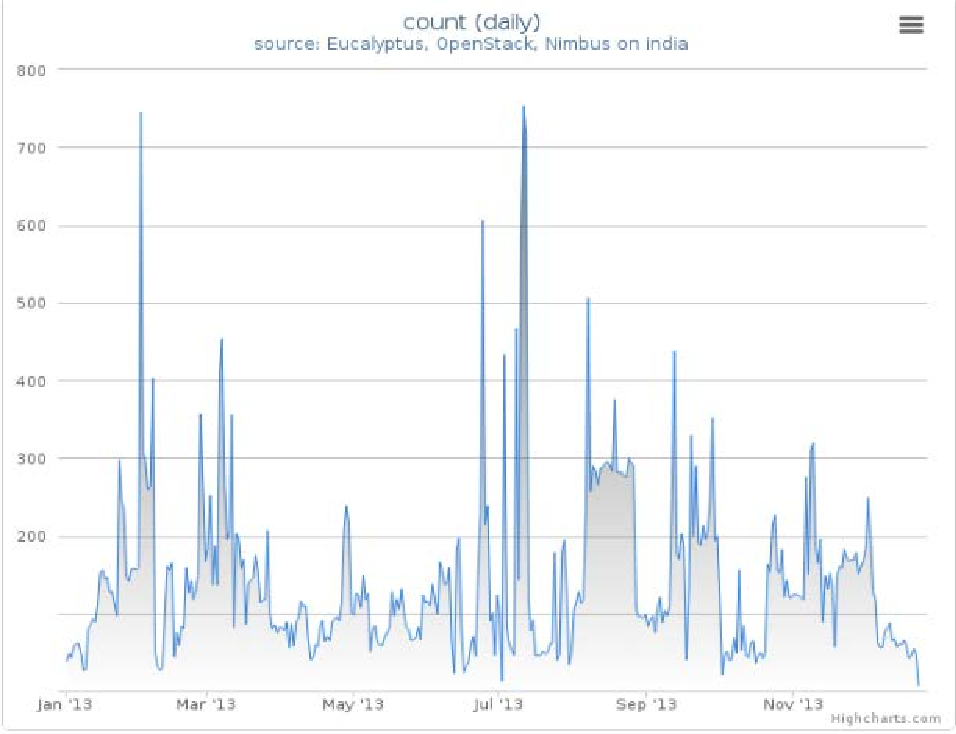
\includegraphics[width=1.0\columnwidth]{images/vmcount.pdf} 
  \caption{VM Count daily}\label{F:vmcount-1} 
\end{figure} 

\begin{figure}[h!] 
  \centering 
    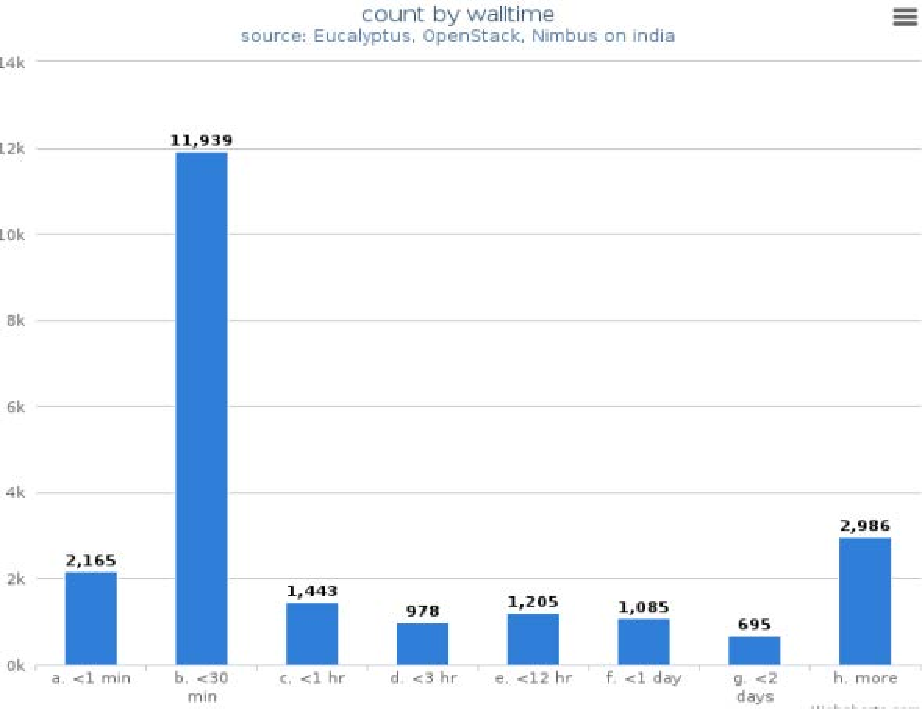
\includegraphics[width=1.0\columnwidth]{images/runtime-histogram.pdf} 
  \caption{VM Count by runtime distribution}\label{F:vmcount-2} 
\end{figure} 

\begin{figure}[h!] 
  \centering 
    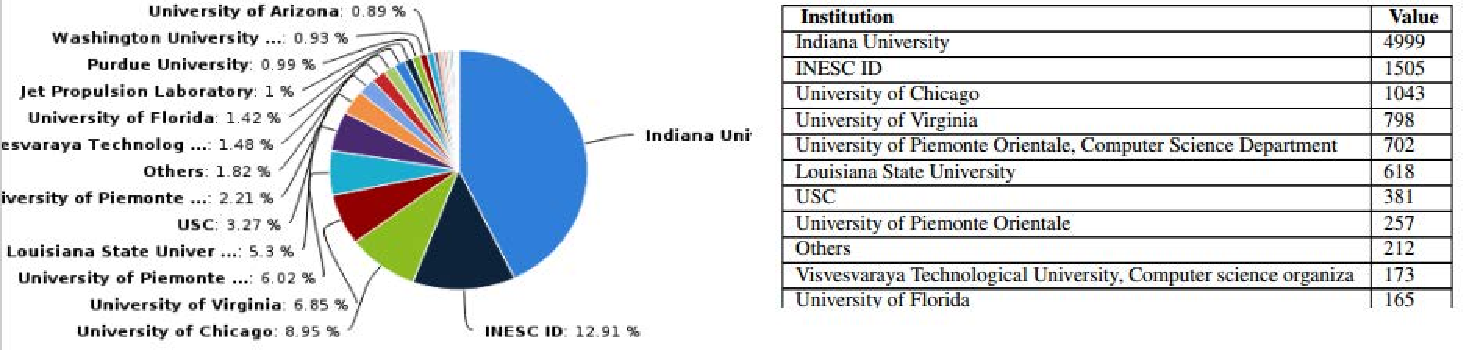
\includegraphics[width=1.0\columnwidth]{images/group-usage1.pdf} 
  \caption{Usage by Institution}\label{F:group-usage-1} 
\end{figure} 
 
\begin{figure}[h!] 
  \centering 
    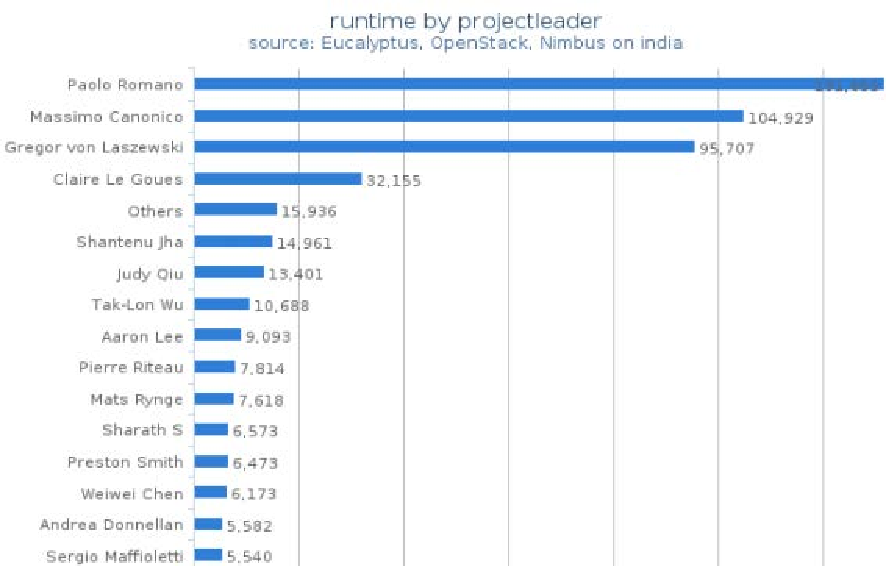
\includegraphics[width=1.0\columnwidth]{images/group-usage2.pdf} 
  \caption{Runtime (Hour) by Project Leader}\label{F:group-usage-2} 
\end{figure} 

\begin{figure}[h!] 
  \centering 
    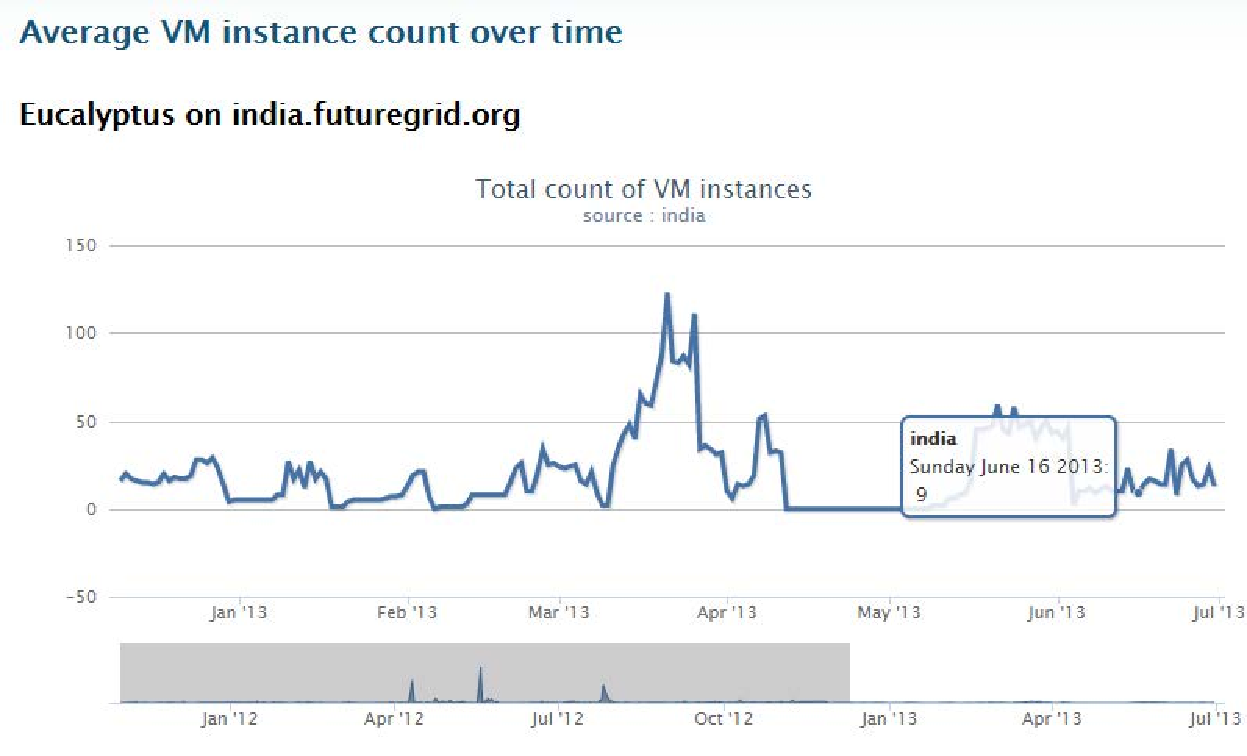
\includegraphics[width=1.0\columnwidth]{images/realtime.pdf} 
  \caption{Real-Time Usage of VM instances}\label{F:realtime-2} 
\end{figure} 
 
\subsection{Sample Reports}

\gregor{complete this section}

Sample report information from FutureGrid is available as html
\cite{LeeFGresourceWeb} or as PDF \cite{LeeFGresource}

\subsection{Error and Alert Reporting}

\begin{table*}[htb]
\caption{Error Metrics}
\begin{scriptsize}
\label{T:metrics}
\bigskip
\begin{center}
\begin{tabular}{lp{0.1\textwidth}p{0.1\textwidth}p{0.1\textwidth}p{0.4\textwidth}}
Metric & Group & Unit & Purpose & Sample \\
\hline
Error Rate &
host, project, or term &
Percentile &
Measure Availability &
2\% errors in i57 host, 4\% errors in April 2015 \\
\hline
Error Count &
host, project, or term &
Count & 
Identify Issues &
399 User Errors (5xx), 133 errors of Instance type\'s disk is too small for requested image (501) \\
\hline
Debug &
host, project, or term &
Count &
Troubleshooting &
133 times failed of \_build\_instance() function in manager.py with error code 5xx \\
\hline
Usage Alert &
VM, CPU, RAM or Disk &
Count or Size &
Notify Limit &
168 of 180 VMs used (93\% used) \\
\hline
Trace Resource  &
VM, CPU, RAM or Disk &
Count or Size &
Inform status &
120/168 free/avail disks \\
\hline
\end{tabular}
\end{center}
\end{scriptsize}
\end{table*}

Cloudmesh Metrics reads system and application logs to generate error
reports. If there are error messages stored in the database, Cloudmesh
Metrics can lookup the database to collect the messages. Error
information collected are stored in the Metrics database.


\begin{table*}[htb]
\caption{Basic Concept of Metric}
\begin{scriptsize}
\label{T:BCmetrics}
\bigskip
\begin{center}
\begin{tabular}{p{0.1\textwidth}p{0.1\textwidth}p{0.3\textwidth}p{0.4\textwidth}}
Name & Unit & Type of Value & Refresh Interval (Measuring time) \\
\hline
Runtime &
hour, min, sec &
cumulative,
aggregation &
event-triggered \\
\hline 
running jobs &
count &
delta, 
(change from the previous value) &
time-triggered e.g. 5 secs, 5 mins\\
\hline
CPU, Memory, Load &
Percentage &
gauge,  
(standalone value relating only to the current duration) &
time-triggered e.g. 5 secs, 5 mins\\
\hline
\end{tabular}
\end{center}
\end{scriptsize}
\end{table*}


\begin{table*}[htb]

\caption{System Performance Metric (OS Level)}
\begin{scriptsize}
\label{T:SPmetrics}
\bigskip
\begin{center}
\begin{tabular}{p{0.15\textwidth}p{0.3\textwidth}p{0.1\textwidth}p{0.1\textwidth}p{0.1\textwidth}p{0.1\textwidth}}
Metric & Description & Type & Level & Unit & Example \\
\hline
CPU Utilization &
Percentages of total CPU time &
System Monitoring &
Operating System & 
Percentage & 
vmstat \\
\hline
I/O Read &
Read operations on disks &
&
&
Count or Bytes &
iostat \\
\hline
I/O Write &
Write operations on disks &
&
&
Count or Bytes  &
\\
\hline
Network In &
Received bytes to network interfaces &
&
&
Bytes &
\\
\hline
Network Out &
Sent bytes from network interfaces &
&
&
Bytes &
\\
\hline
\end{tabular}
\end{center}
\end{scriptsize}
\end{table*}


\begin{table*}[htb]
\caption{Network Monitoring Features (source from wikipedia)}
\begin{scriptsize}
\label{T:NMmetrics}
\bigskip
\begin{center}
\begin{tabular}{p{0.15\textwidth}p{0.4\textwidth}p{0.1\textwidth}p{0.1\textwidth}}
Metric (legend) & Description & Ganglia & Nagios \\
\hline
Trending &
Provides trending of network data over time &
Yes &
Yes \\
\hline
Trend Prediction &
The software features algorithms designed to predict future network statistics &
No &
No \\
\hline
Auto Discovery &
The software automatically discovers hosts or network devices it is connected to &
Via gmond check in &
Plugin \\
\hline
Agentless & 
The product does not rely on a software agent that must run on hosts it is monitoring so that data can be pushed back to a central server. &
No &
Supported \\
\hline
SNMP &
able to retrieve and report on SNMP statistics &
Plugin &
Plugin \\
\hline
Syslog &
Able to receive and report on Syslogs &
No &
Plugin\\
\hline
\end{tabular}
\end{center}
\end{scriptsize}
\end{table*}


\begin{table*}[htb]
\caption{Metrics for Cloud Computing}
\begin{scriptsize}
\label{T:NMmetrics}
\bigskip
\begin{center}
\begin{tabular}{llll}
Metric & Cloud Platform & Purpose & Related Service \\
\hline
CPU Utilization &
IaaS, PaaS &
Performance &
Scale Up/Down \\
\hline
Task completion time &
PaaS &
Performance &
\\
\hline
Number of VMs &
IaaS &
Traffic &
Scale Up/Down \\
\hline
VM sizes (flavors) &
IaaS &
Capacity &
\\
\hline
\end{tabular}
\end{center}
\end{scriptsize}
\end{table*}
\cite{aceto2013cloud}

\begin{table*}[htb]
\caption{System Monitoring on Cloud platforms}
\begin{scriptsize}
\label{T:SMmetrics}
\bigskip
\begin{center}
\begin{tabular}{p{0.1\textwidth}p{0.1\textwidth}p{0.1\textwidth}p{0.1\textwidth}p{0.1\textwidth}p{0.1\textwidth}p{0.1\textwidth}}
Metric & AWS & GCE & Azure & OpenStack & HP Cloud (Eucalyptus) & Nimbus \\
\hline
CPU Utilization & Yes & TBD & TBD & TBD & TBD & TBD \\
\hline
I/O Read & Yes & TBD & TBD & TBD & TBD & TBD \\
\hline
I/O Write & Yes & TBD & TBD & TBD & TBD & TBD \\
\hline
Network In & Yes & TBD & TBD & TBD & TBD & TBD \\
\hline
\end{tabular}
\end{center}
\end{scriptsize}
\end{table*}

%%%%%%%%%%%%%%%%%%%%%%%%%%%%%%%%%%%%%%%%%%%%%%%%%%%%%%%%%%%%%%%%%%%%%%
\section{MONITORING TOOLS AND SERVICES}\label{S:tools}
%%%%%%%%%%%%%%%%%%%%%%%%%%%%%%%%%%%%%%%%%%%%%%%%%%%%%%%%%%%%%%%%%%%%%%

\subsection{IaaS}

\subsubsection{OpenStack}


Openstacks Ceilometer provides a service for measuring usage data from openstack components to achieve monitoring and metering purposes. Ceilometer acquires measurements across current OpenStack components such as Nova (compute), Network, and Storage (swift). Next to an API it also provides a command line tools to retrieve usage statistics. However in deployments such commands are typically limited by policy to system administrators. By default it provides hourly information for compute utilization; instance type; availability zone; cpu core; memory size; nova volume block device type and availability zone; Network; data transfer (in / out), availability zone; external floating ip; Storage (Swift); disk size used; and data in/out.

There are four basic components to Ceilometer:

\begin{description}
\setlength\itemsep{-2pt} 

\item[\it Agents.] Agents run on each compute node and polls resources utilization statistics.

\item[\it Collector:] A collector runs on management servers to manage the message queues for data coming from the agent. Metering data are stored to the openstack data store and a notification message are delivered to the Openstack messaging bus once they are processed.

\item[\it Data store:] is a place of collected data. It provides interaction with the collector and a api server.

\item[\it API server:] runs on management servers to provide statistics about the measured data.

\end{description}

Production scale metering is estimated to have 386 writes per second and 33,360,480 events a day, which would require 239 Gb of volume for storing statistics per month~\cite{Barcet12}.

The OpenStack Orchestration program, Heat, provides an autoscaling service while leveraging Ceilometer. It is similar to Amazons CloudFormation.  This integration of Heat and Ceilometer allows users to develop services that provide better resource utilization. This is similar to the combination of the AWS Auto Scaling and AWS CloudWatch to provide the autoscaling service based on monitoring values~\cite{Abaakouk13}.

In addiction to ceilometer the command line tools provided by OpenStack Compute (Nova) offer elementary usage statistics, but also inform users about quota and API call limitations.  For more detailed information about resource usage users will need to use the information exposed with ceilometer.  Examples of the information includes host information as depicted in Figure~\ref{F:host-describe} and usage data as depicted in Figure~\ref{F:host-describe}.


\begin{figure}[htb]
\begin{scriptsize}
\begin{verbatim}
    $ nova host-describe i40
    +--------+------------+-----+-----------+---------+
    |  HOST  | PROJECT    | cpu | memory_mb | disk_gb |
    +--------+------------+-----+-----------+---------+
    | i40    | (total)    | 8   | 24100     | 2698    |
    | i40    | (used_max) | 10  | 19456     | 180     |
    | i40    | (used_now) | 10  | 18944     | 180     |
    | i40    | project1   | 1   | 2048      | 20      |
    | i40    | project2   | 8   | 16384     | 160     |
    | i40    | project3   | 1   | 512       | 0       |
    +--------+------------+-----+-----------+---------+
\end{verbatim}
\vspace{-20pt}
\end{scriptsize}

\caption{Display a summary of resource usage of the devstack-grizzly host}
\label{F:host-describe}

\begin{scriptsize}
\begin{verbatim}
    $ nova usage-list
    Usage from 2014-02-14 to 2014-03-15:
    +--------+---------+-------------+---------+-----------+
    | Tenant | Instan- | RAM         | CPU     | Disk      |
    | ID     | ces     | MB-Hours    | Hours   | GB-Hours  |
    +--------+---------+-------------+---------+-----------+
    | user1  | 17      |  6840394.43 | 3340.04 |  66800.73 |
    | user2  | 17      |   185683.06 |   90.67 |   1813.31 |
    | user3  | 1       |   932256.36 |  455.20 |   9104.07 |
    | user4  | 26      |  4947215.08 | 2415.63 |  48312.65 |
    | user5  | 5       | 18644854.23 | 9103.93 | 182078.65 |
    +--------+---------+-------------+---------+-----------+
\end{verbatim}
\vspace{-20pt}
\end{scriptsize}

\caption{Summary statistics for tenants}
\label{F:host-describe}

\end{figure}


Internally usage data for Ceilometer and the nova command line tools is provided by OpenStack Notification System. The notification system can be configured to emit events either through nova's logging facility, or send them to a series of AMQP queues (one per notification priority). System usages are emitted as notification events with the INFO priority. Different types of usage events are distinguished via the notifications \verb|event_type|, which is a hierarchical dotted string such as \verb|compute.instance.create|, which allows usages to be easily grouped for aggregation. Usage notifications can be immediate (created when a specific increment of usage occurs, such as creation of an instance) or periodic (generated by a periodic task, like a cron job) and cover usage for a certain time period. A notification includes attributes such as id, priority, event type, and timestamp associated with a notification data payload as a json-formatted key-value pair ~\cite{SystemUsageData}.  Through this set of information custom parsers and information queries can be generated. However it does require policies to be set up to gain access to this information.

\subsubsection{Eucalyptus}

Eucalyptus provides a to several Amazon services compatible private cloud.  It offers resource usage information through external monitoring tools such as Nagios and Ganglia.  To enhance system management, Eucalyptus provides nowadays summary reports about resource allocation and status. There are commands line tools for generating reports for eucalyptus cloud that start with eureport- in the Cloud Controller (CLC) and eucadw- in the data warehouse. The reports provide usage data for understanding how cloud resources are utilized and being used via simple command line tools. eureport-generate-report is a main command to get access usage data. Various type of resources can be measured such as elastic-ip, instance, s3, snapshot, and volume when eureport-generate-report is ran with a report type option. The Eucalyptus data warehouse is a place to keep all usage data coming from CLC. External programs can get access to the usage data from the data warehouse instead of CLC directly. It may reduce impact of pulling usage information from cloud when it performs its cloud duties~\cite{Euca2ools14}.  Previously Eucalyptus did not have a strong monitoring framework and as part of FutureGrid we developed a system that parses log file events on the management node to provide them. In future we need to evaluate if the existing Eucaluptus monitoring features could replace this framework. However, as the usage demand of Eucalyptus has almost diminished, we have in FutureSystem discontinued the use of Eucalyptus. University of Buffalo is in the process of deploying a Eucalyptus cloud and we hope the integration of Eucalyptus data into a heterogeneous metrics framework can be continued at that time. At this time we are not aware of any other new Eucalyptus cloud deployments.

\subsubsection{Azure}

Microsoft Windows Azure is a cloud computing platform used to build, host and scale web applications through Microsoft data centers~\cite{azure11}. The platform contains various on-demand services hosted in Microsoft data centers. These services are provided through three products.

\begin{description}
\setlength\itemsep{-2pt} 

\item[\it Windows Azure:] an operating system that provides scalable compute and storage facilities.

 \item[\it SQL Azure:] a cloud based, scale out version of SQL server.

 \item[\it Windows Azure AppFabric:] a collection of services supporting applications both in the cloud and on premise.

\end{description}

The System Center Monitoring Pack for Windows Azure application is according to Microsoft the most cost effective and flexible platform for managing traditional data centers, private and public clouds, and client computers and devices~\cite{MonitoringPackAzure11}. It provides monitoring of availability and performance for Windows Azure applications. It provides a unified management platform where multiple hypervisors, physical resources, and applications can be managed in a single offering. From a single console view, the IT assets like network, storage and compute can be organized into a hybrid cloud model spanning the private cloud and public cloud services. The monitoring pack runs on a specified agent and uses Windows API.s to remotely discover and collect information about a specified Windows Azure application. By default, the monitoring is not enabled. Therefore, the discovery must be configured by using the Windows Azure Application monitoring template for each Windows Azure Application to be monitored. The following functionalities are provided by the Monitoring Pack for Windows Azure Applications:

\begin{itemize}
\setlength\itemsep{-2pt} 

 \item Discovers Windows Azure applications.
 \item Provides status of each role instance.
 \item Collects and monitors performance information.
 \item Collects and monitors Windows events.
 \item Collects and monitors the .NET Framework trace messages from each role instance.
 \item Grooms performance, event, and the .NET Framework trace data from Windows Azure storage account.
 \item Changes the number of role instances.
\end{itemize}

Implementing monitoring means, launching the diagnostic instance and this instance will collect the data and at the interval user wants. The collected data will be copied to an Azure Table to record information for performance counters and windows event logs.  The performance monitoring can be enabled by direct implementation or using tools such as powershell cmdlets for Windows Azure~\cite{cmdlets} or the Azure Diagnostics Manager 2 from Cerebrata~\cite{cerebrata}.

By using these tools one instance of Windows Azure is configured to collect some performance counters without modifying the application code. The performance data will be collected by the Azure Diagnostic Monitor and moved at the interval user specified. Hence the user can use this diagnostic data for debugging and troubleshooting, measuring performance, monitoring resource usage, traffic analysis and capacity planning, and auditing. Diagnostic data is not permanently stored unless user transfers the data to the Windows Azure storage emulator or to Windows Azure storage. After the data is transferred to storage it can be viewed with one of several available tools. To collect Windows Event logs in a Windows Azure application, the Event logs data source must be configured. Access is controlled by authentication access control.  The monitoring data can be visualized using System Center Operation Manager Console. From Operation Manager, user can create custom dashboard or publish graphs on SharePoint to people who do not have the SCOM console.

\subsubsection{Amazon}

\paragraph{Amazon CloudWatch}

Amazon CloudWatch (ACW) \cite{cloudwatch2013monitoring} monitors Amazon Web Services (AWS) resources and the applications users run on AWS in real-time.  ACW is a metrics repository. The AWS products ingest metrics into the repository, and users retrieve statistics based on those metrics.  Metrics are time-ordered sets of data points, are isolated from one another in different namespaces so that metrics from different applications are not mistakenly aggregated into the same statistics. Users retrieve statistics about those data points as an ordered set of time-series data. Over the time value is important for metrics since it contains historical changes in it. An API is provided to interface programmatically.

CloudWatch allows notification to alert users and auto scaling (automatically make changes) to the resources you are monitoring based on rules that you define. Hence, CloudWatch can manage thresholds to send a notification to users via email or text messages, and even more, apply changes with a pre-defined settings such as increasing virtual instances or diminishing. System-wide visibility into resource utilization, application performance, and operational health can be provided on a users services. However insight into the underlaying IaaS framework is not sufficiently provided as is tha case in academic private clouds.

\subsubsection{Rackspace Cloud Monitoring}

Rackspace Cloud Monitoring is an API driven monitoring system which allows administrators to use or create APIs depending on their needs which can send notifications to any device including mobile devices. This allows administrators to be on top of their Rackspace-hosted infrastructure which includes websites, protocols, and ports.

\subsubsection{Google Cloud}

Google launched Cloud Monitoring in 2014 after the acquisition of Stackdriver, a software company that developed monitoring services in the cloud. Google Cloud Monitoring (GCM) provides performance data of cloud resources and sends notifications if issues occur based on a user defined alerting policy.  Monitoring is available in Google App Engine, Compute Engine, Pub Sub, Cloud SQL and Cloud Storage with health check, log tracing on the web-based Cloud Monitoring Console according to the Cloud Monitoring website~\cite{GCM}.  Additional metrics such as memory or disk usage can be collected by the Monitoring Agent which requires to be installed in a VM instance. Google offers Monitoring for free during its Beta release.

\subsection{HPC}

Monitoring in high-performance computing has similar factors as described earlier. A number of existing tools support monitoring and metrics for HPC computing. Some of them are directly build into the queuing system. We describe a selected number of tools and services next.

\subsubsection{XDMoD}

XDMoD (XSEDE Metrics on Demand) \cite{las14cloudmeshmultiple,las14Impact,las12xdmod-kernel} is developed as a successor to UBMoD (University Buffalo Metrics on Demand) while trageting firstly the XSEDE resource providers. Most recently an open source version can however be deployed at non XSEDE based resource providers. It is a tools for collecting and mining statistical data from cluster resource managers such as Torque\cite{staples2006torque}, Maui\cite{jackson2001core}, Moab\cite{computing2012moab}, OpenPBS \cite{teambatching}, SGE\cite{gentzsch2001sun} and Slurm \cite{jette2010slurm} commonly found in high-performance computing environments. XDMod has three fundamental components: a metrics repository (e.g. a Data Warehouse), a RESTful API, and a web-based application (Portal).  Its web graphical user interface provides rich set of tools to expose various statistics with different type of charts and tables while communication through a RESTful API ~\cite{CPE:CPE2871,Furlani:2013:UXF:2484762.2484763}.

\subsubsection{Nagios}

Nagios \cite{barth2008nagios} is a web based Linux monitoring systems allowing to monitor availability and response time of network services, usage of system resources like CPU load, RAM allocation etc., number of logged in users and so on. The main Nagios server collects information from Linux, BSD, Windows hosts or Cisco devices through Nagios clients (agents), and records their states. A web interface is provided to expose the information to authorized users.  Nagios generates a notification in case of any outage detected or any anomaly through wide range of alert methods. They can be forwarded via e-mail, sms, chat messages and phone call notifications. As Nagios monitors states but it typically does not expose graphs such as network interface usage.

\subsubsection{Cacti}

Cacti is a network monitoring tool using the simple network management protocol (SNMP). It is similar to other tools such as Nagios \cite{barth2008nagios} and Ganglia. It uses RRDtool \cite{oetiker2005rrdtool} as a DBMS to provide a round robin visualization of the monitored information. Since it supports polling, monitoring data via shell scripts, php, or c-based executable is possible. t can be extended to measure other resources besides network traffic.

\subsubsection{Zabbix}

Zabbix is an open source monitoring service for networks and servers while accessing information via a number of standard protocols such as SNMP \cite{case1990simple}, IPMI \cite{dell2009ipmi}, TCP, \cite{cerf2005protocol} and JMX \cite{perry2002java}. The centralized server of Zabbix collects monitoring data through several Zabbix agents installed on desirable hosts and other servers. The information is store in a database and displayed through a web interface that can create reports on-demand. The agents To support cloud monitoring, Zabbix active agent auto-registration enables monitoring cloud instances on IaaS such as Amazon Web services, and OpenStack.

\subsubsection{Zenoss}

Zenoss (Zenoss Core) provides a unified resource management service which manages applications, networks, servers, and storage. It allows to monitor physical or virtual systems including the public, private and hybrid clouds. It is built on top of the Zope object-oriented web application server, and using RRDtool with MySQ. It can collect information using SNMP, SSH, WMI and log files e.g. syslog. Zenoss provides additional features with other monitoring mechanisms such as Perfmon, JMX, and VM API (e.g. VMware API) in the enterprise version. A key feature of Zenoss is model-driven monitoring allowing to automatically discover, configure and monitor services. As a communication tool, Zenoss utilizes the Twisted Perspective Broker (PB) \cite{PerspectiveBroker} instead of AMQP typed messaging system such as RabbitMQ. PB is an an asynchronous, event-driven with co-operative multi-tasking which is a deferred object.

\subsubsection{Inca}

Inca is monitoring software for watching user-level activities and measuring performance on a Grid including detecting errors~\cite{inca}. The executable program, Inca reporter, collects performance data from a system and Inca web interface provides detailed information about the measured data. XSEDE uses Inca for monitoring GRAM usage, CA and CRL validity and resource registration in MDS according to the project description page~\cite{inca-xsede}.  FutureGrid project used Inca for measuring performance of FutureGrid software and hardware with 196 Inca reporters for testing FutureGrid services and clusters~cite{inca-futuregrid}. Inca is used on the XSEDE resources Keenland \cite{keeneland}\cite{keeneland-xsede} and Darter \cite{darter-nics}.


\subsubsection{Ipm} 

``Integrated Performance Monitoring (IPM) is a portable profiling infrastructure for parallel codes. It provides a low-overhead performance summary of the computation and communication in a parallel program.'' \cite{Shan:2010:ProgModels,Fuerlinger:2010:PetascaleIPMP,ipm-github,ipm10} Ipm is used on the XSEDE resource Stampede \cite{stampede-tacc}.

\subsubsection{PAPI}

``PAPI provides the tool designer and application engineer with a consistent interface and methodology for use of the performance counter hardware found in most major microprocessors. PAPI enables software engineers to see, in near real time, the relation between software performance and processor events. In addition Component PAPI provides access to a collection of components that expose performance measurement opportunites across the hardware and software stack.''  PAPI is used obn the XSEDE resource Stampede \cite{stampede-tacc}.

\subsubsection{Gold}

There is a small number of accounting software to provide metered resource utilization in open source cloud platforms. Those tools such as Gold accounting Manager~\cite{jacksongold,gold-allocation} are very simple and are supposed to support system administrators not cloud users. However, Gold is no longer supported by the developers.


\subsubsection{XRAS}

The XSEDE Resource Allocation Service (XRAS) is an allocations environment for managing the submission, review, and awarding of resource allocations. It is targeted to better serve the XSEDE infrastructure than its predecessors. It streamlines the allocations processes across a broad set of cyber infrastructure investments. XRAS is designed as a software-as-a-service through a set of common tools and interfaces enhanced by flexible mechanisms that allow clients to tailor the environment to meet the needs of their process \cite{hart2014xras}.


%%%%%%%%%%%%%%%%%%%%%%%%%%%%%%%%%%%%%%%%%%%%%%%%%%%%%%%%%%%%%%%%%%%%%%
\section{CLOUDMESH METRICS SERVICES AND FRAMEWORK}\label{S:cloudmesh}
%%%%%%%%%%%%%%%%%%%%%%%%%%%%%%%%%%%%%%%%%%%%%%%%%%%%%%%%%%%%%%%%%%%%%%

Cloudmesh Metrics extends our cloudmesh framework \cite{las14cloudmeshmultiple} by integrating a metrics framework for monitoring essential IaaS metrics. It can handle handling multiple heterogeneous cloud platforms, to provide measurement of usage data about cloud resources.  It collects usage data directly from various cloud management services and integrates them into a single report. This framework was extensively used in FutureGrid~\cite{las2010gce,las12fg-bookchapter} and its use is continued in FutureSystems \cite{??}. It has served as integrator to three different IaaS frameworks, namely, Eucalyptus, OpenStack, and Nimbus. It has served to provide integrated information of at least eight different cloud deployments on various hosts in FutureGrid and FutureSystems.  The native usage data from different clouds are integrated into the Metrics database. Analysis of this data can be integrated into different report formats including PDF, and HTML. An API and a command line interface is available to customize reports while exposing them also through a REST interface. A Web interface provides a number of predesigned reports. Interactivity to min the graphs~\cite{highsoft2012highcharts} is provided through java script enabled charts or tables.

\subsection{Design}

The design of the cloudmesh metrics framework allows the mashup of information from various data sources including cloud management databases and log files. This mashup provides us with a rich data set supporting sophisticated analysis that may spawn multiple information sources.  The system has been used in FutureGrid to support metric information from multiple IaaS service providers from various FutureGrid partner sites, for more than 400 projects and over 2800 members as of end of 2014 ~\cite{las14cloudmeshmultiple}.

Figure~\ref{F:fig7} shows a layered architectural view of the Cloudmesh Metrics service and how it interfaces with various IaaS frameworks.

Cloudmesh Metrics consists of four components: (1) Metric Collector: a measuring tool of resource allocation, (2) Cloudmesh Metric Shell providing a CLI tool to define metrics and collect usage data, (3) Cloudmesh Metric Portal and Report providing a visualization tool to provide graphical representative of the data, and (4) a Web Service APIs to support other applications e.g. scheduling and dynamic provisioning.

\begin{figure*}[htb] 
\begin{center}
 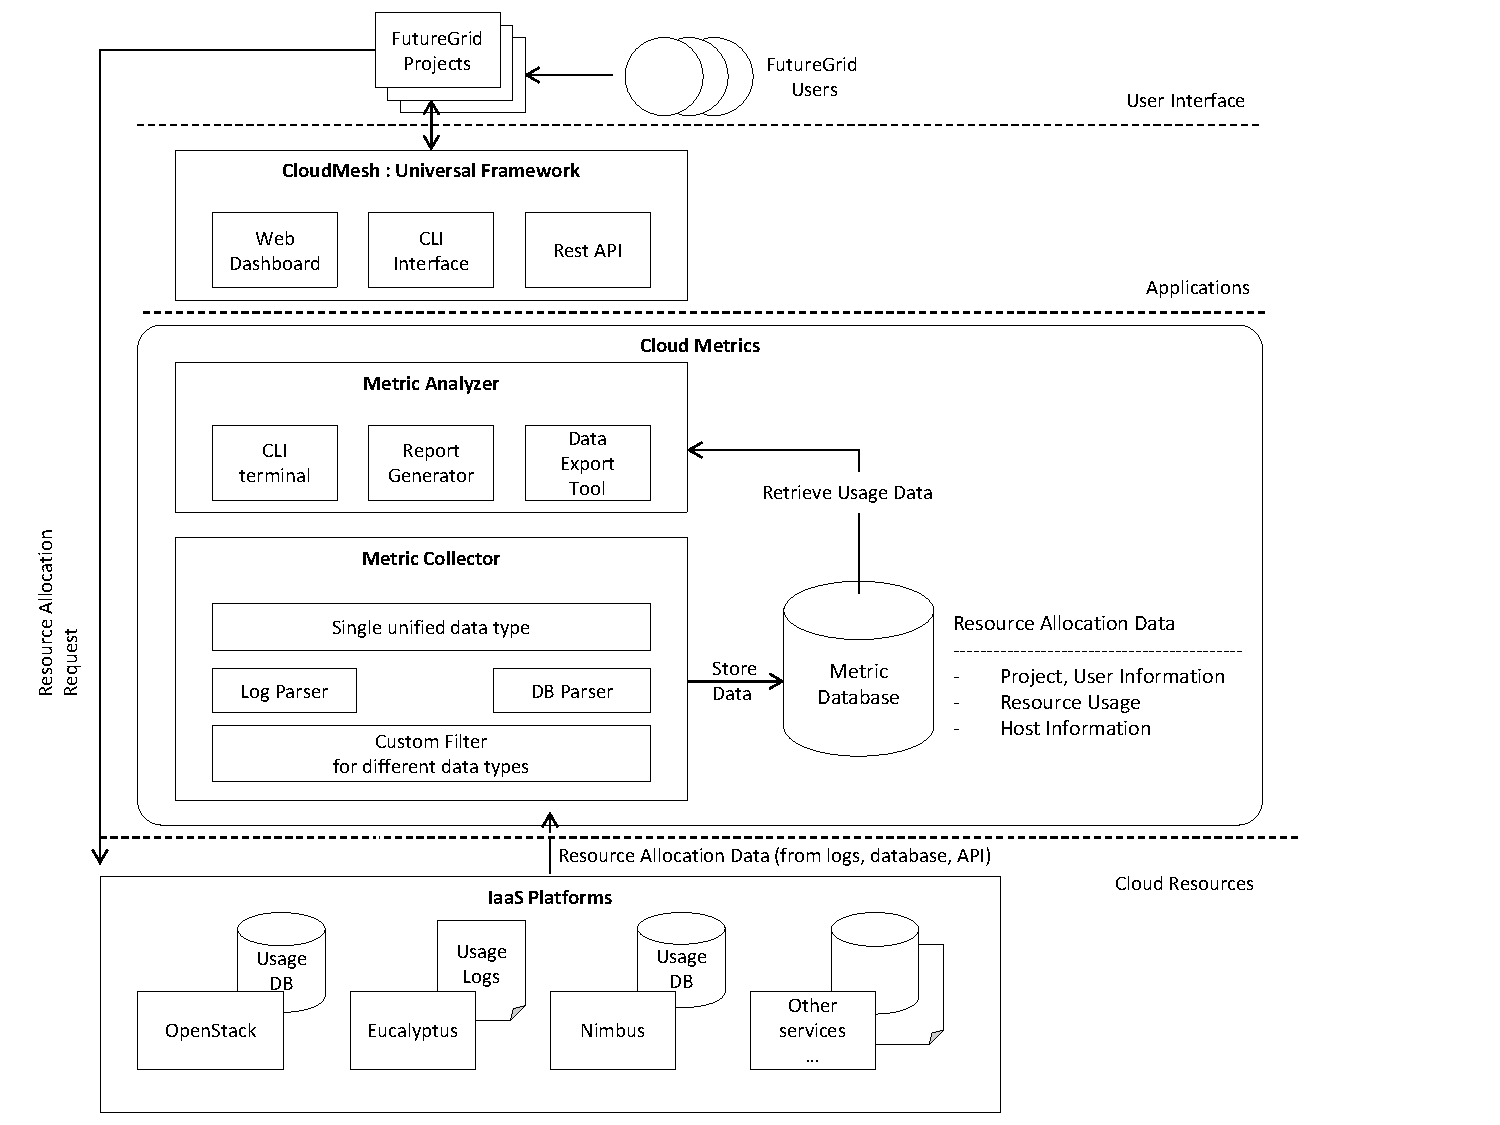
\includegraphics[width=1.0\textwidth]{images/system_overview.pdf} 
\end{center}
  \caption{Overview of Cloud Metrics \hyungro{we need to redraw, can
      this be dne in ppt or omni graffel}}\label{F:fig7} 
\end{figure*} 

The Metric Collector enables collecting usage data allocated from IaaS cloud platforms such as Eucalyptus, Nimbus, and OpenStack including HPC from TORQUE.  A log parser extracts data from log messages of IaaS platforms and transforms them into metrics.  The metrics are then stored into a database that allows exposing the data as JSON objects via API calls.  The collecor enables also real-time monitoring and statistics. Data can be integrated from OpenStack MySQL databases or Nimbus sqlite3 to the unified database. Fro Eucalyptus we obtained most of the information through its log files as at the time Eucalyptus did not provide a sophisticated monitoring or metrics framework beyond the available logging facility. Account information such as a user name and a project associated with are also imported to the main database so the overall usage data can be viewed for vm instances and jobs launched on FutureGrid resources via LDAP.

To keep the load on the original services minimal, we pull data on regular intervals from these production systems. Other mechanisms such as access to replicated databases could easily be supported.

\subsection{Selected Analysis with Cloudmesh Metrics}

To showcase the usefulness of the system we present some simple examples from our operation of FutureGrid and FutureSystems spawning multiple years of production deployment. We early found that a simple summary view provides valuable input to management and funders.  Furthermore the automatically generated reports at predefined intervals serve the required quarterly reporting. An examples of such summaries are provided in Figure \ref{F:fig8}. Real time information about virtual machine usage is depicted in \ref{fig:9}.

\begin{figure}[htb] 
  \centering 
    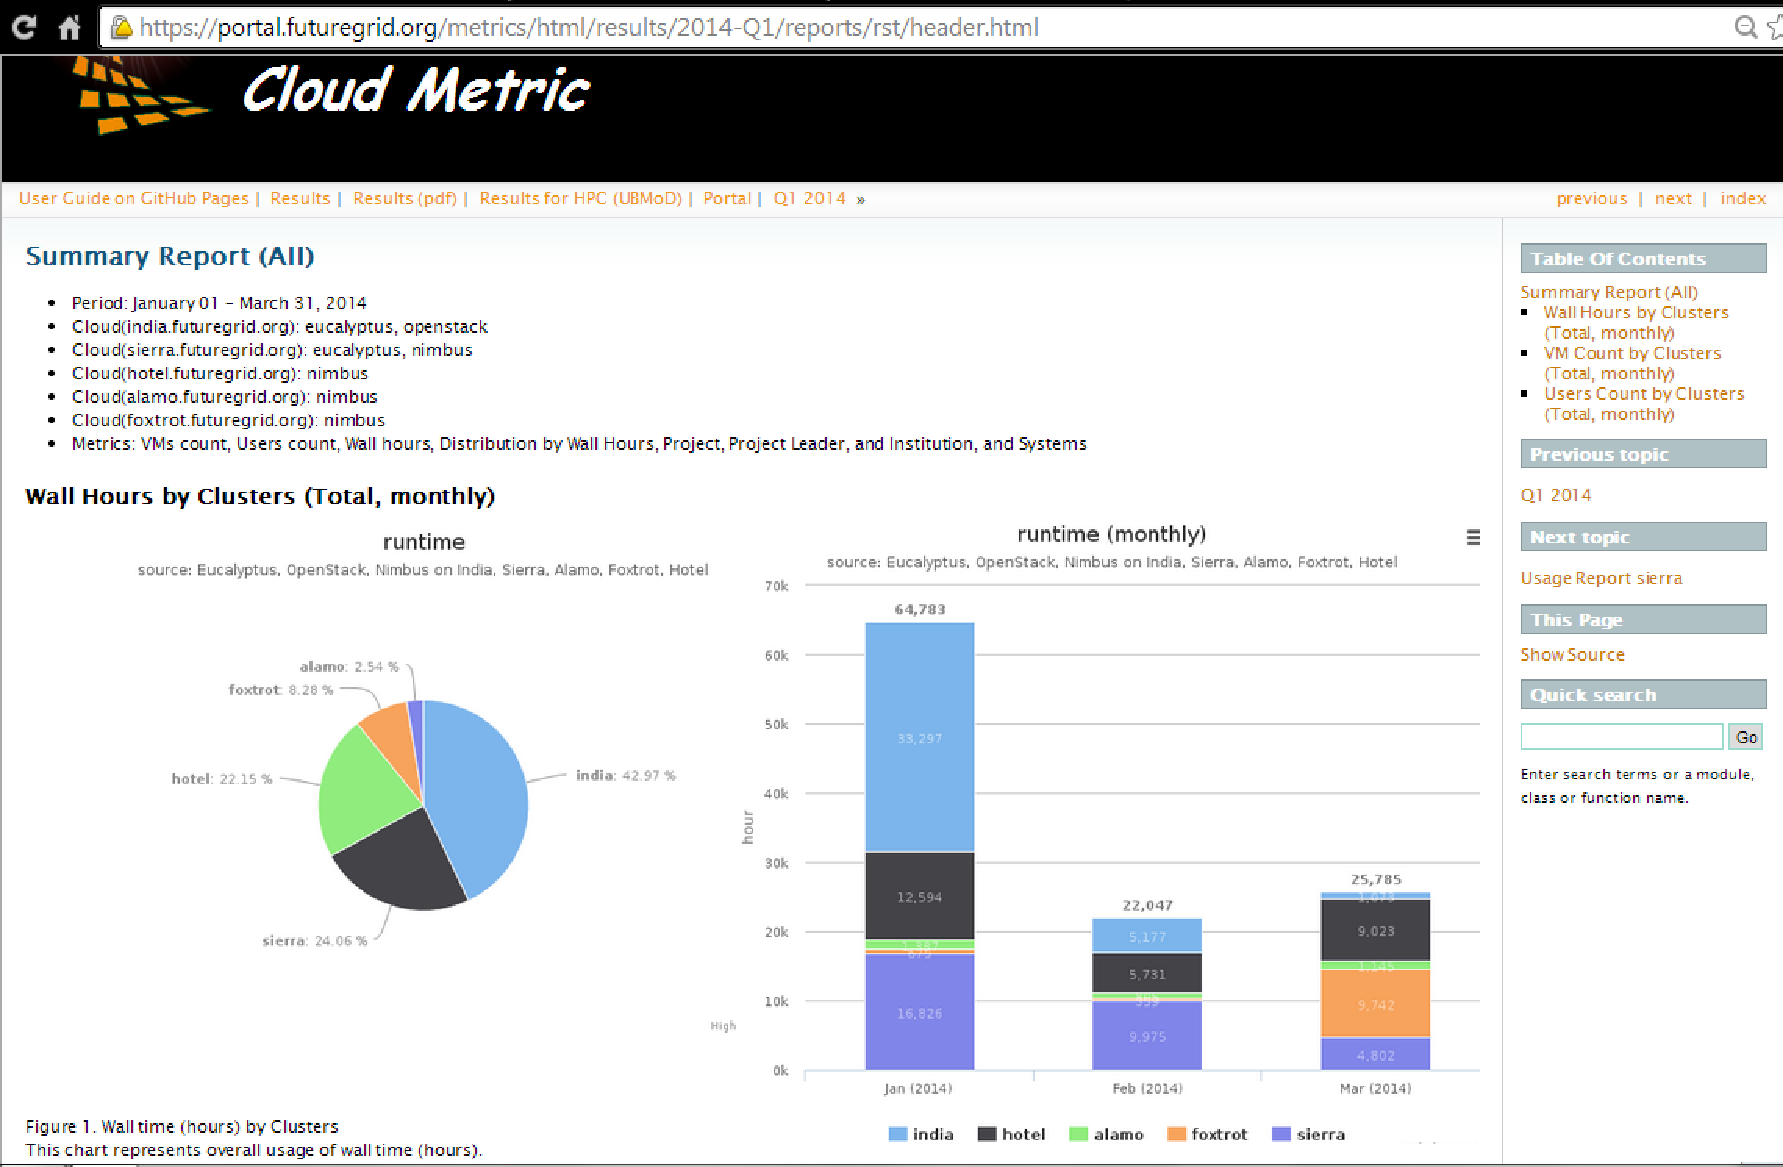
\includegraphics[width=1.0\columnwidth]{images/metrics-portal.pdf} 
  \caption{Cloud Metrics Portal pie chart and stacked bar chart represent monthly usage of FutureGrid resources. Summary of regional clusters and different IaaS cloud platforms are displayed with various charts and different terms including monthly, quarterly and yearly.}\label{F:fig8} 
\end{figure} 

\begin{figure}[htb] 
  \centering 
    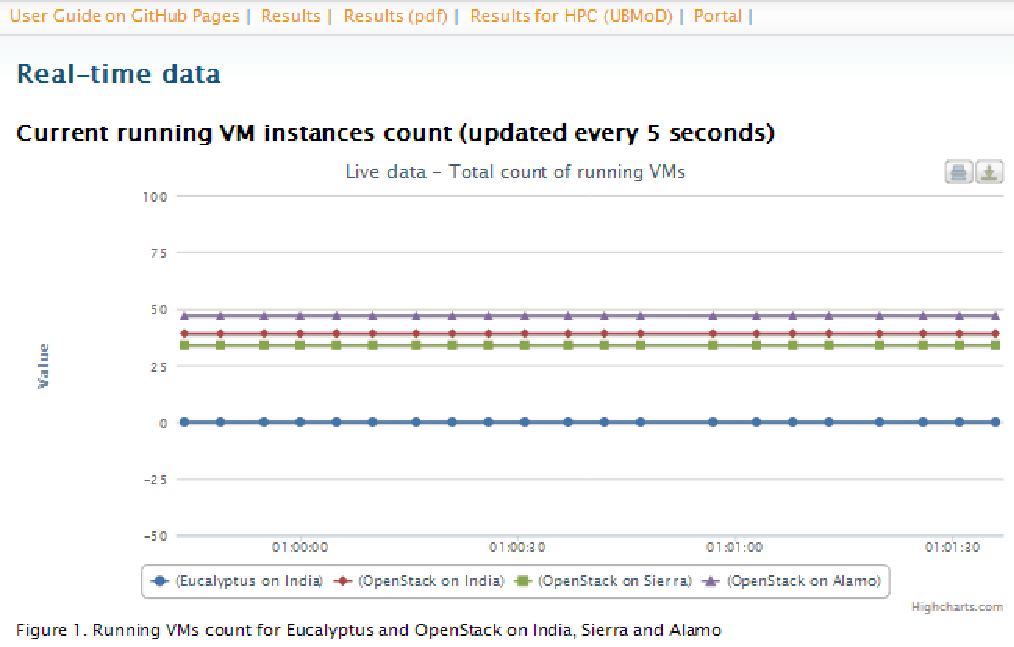
\includegraphics[width=1.0\columnwidth]{images/metrics-portal-realtime.pdf} 
  \caption{Real-time usage report on Cloud Metrics Portal: In every 5 seconds, the line chart is updated with the number of working virtual machine instances.}\label{F:fig9} 
\end{figure} 

Based on the observation on FutureGrid, there is a different pattern between a research project and class work when they acquire cloud resources. Resource allocation of academic coursework shows time dependent request patterns. It shows a surge when there is a class, a lab session, and a project. For example, the undergraduate course for Distributed Systems at Indiana University introduced IaaS in the class and used the IaaS platform for a class project. Figure~\ref{F:fig2} shows a spike in the class and variability until the project due.  Additionally, we have been able to expose to the class lead that despite students attending this class not all students have actually logged into the systems or created VMs. Such information may provide valuable input to the teacher in order to verify group work or avoid academic dishonesty. It also contradicted the demand for the faculty member to ``reserve'' for the entire semester a substantial number of compute resources so they can be exclusively used by the class. Although we observe a spike, the available resources in the overall cloud would have been sufficient to satisfy the user demand.

While we see time dependent use in classes, many research project show in contrast VM instances requests on a more regular basis. An example is found in the Next Generation Sequencing (NGS) in the cloud project on FutureGrid shows relatively consistent resource allocation requested in Figure~\ref{F:fig3}. With a certain period of time, vm instances of this project have been launched without unplanned spike requests. These two examples show different patterns for deploying resources but both cases have a factor to predict loads. The class schedule and the monitoring data for applications can be used to measure the amount of resources and identify incoming requests.  While having this information available through our project registration makes it possible to predict in future similar behavior.  Hence understanding these patterns is important to bring cost effectiveness over on-demand allocation.

\begin{figure}[htb] 
  \centering 
    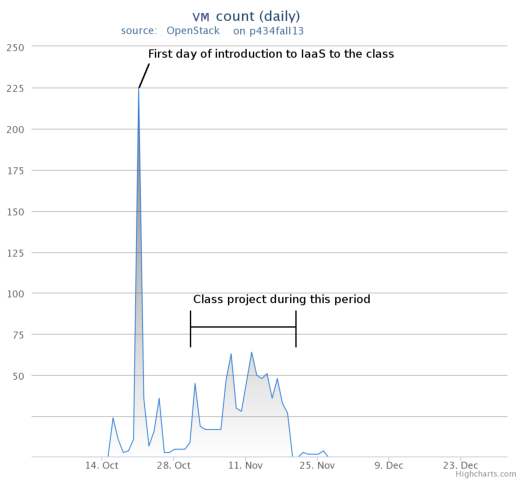
\includegraphics[width=1.0\columnwidth]{images/fig1.pdf} 
  \caption{IaaS Usage data for the Distributed System class at Indiana University*}\label{F:fig2} 
\end{figure} 


% * Based on the class schedule and metrics. Class schedule is here: http://salsahpc.indiana.edu/csci-p434-fall-2013/
% Metrics is here: http://129.79.49.94/accounting/reports/custom/p434fall13/FGResourceReport.pdf

\begin{figure}[htb] 
  \centering 
    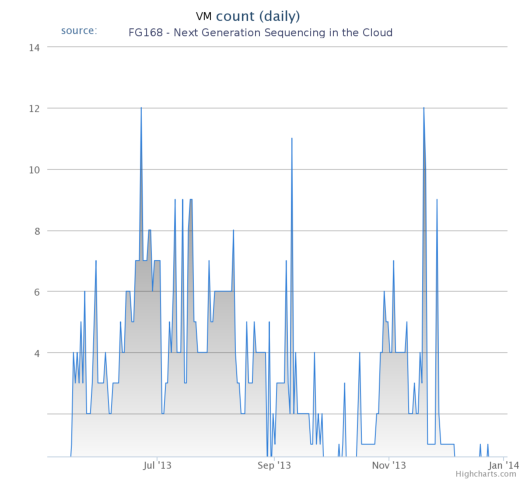
\includegraphics[width=1.0\columnwidth]{images/fig2.pdf} 
  \caption{VM count for Next Generation Sequencing (NGS) in the cloud project}\label{F:fig3} 
\end{figure} 

We can furthermore analyse the data for the class usage as shown in the Gantt chart Figure~\ref{F:fig4}. Here we display the duration of the VMs as used in the class. At the beginning of the class, the gaps between the start and completed dates of the vm instances are small but a large number of instances are initiated. Once the class is became operative, the runtime of vm instances is getting longer and a less number of instances are requested compared to the beginning. This observation tells us that academic projects require training sessions using short running VMs at the beginning of a project to get familiar with using infrastructure and to prepare environments by installing software and datasets.

\begin{figure}[htb] 
  \centering 
    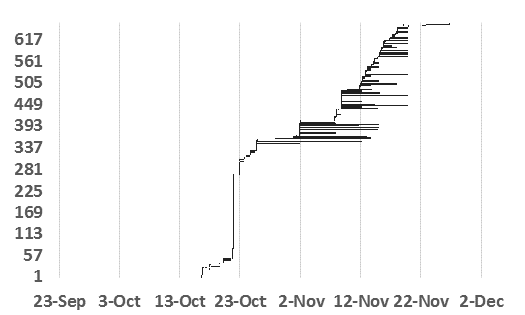
\includegraphics[width=1.0\columnwidth]{images/fig3.pdf} 
  \caption{Timeline for VM walltime}\label{F:fig4} 
\end{figure} 

Another observation is that this particular class had a quite high usage of VMs for administrative purposes by the instructor. Figure~\ref{F:fig5} describes that instructors consumed a large number of vCPU cores before class starts and small tests just before class projects. It indicates that the preparation of courses require extensive load testing on cloud resources to estimate compute capacity needed for applications.

\begin{figure}[htb] 
  \centering 
    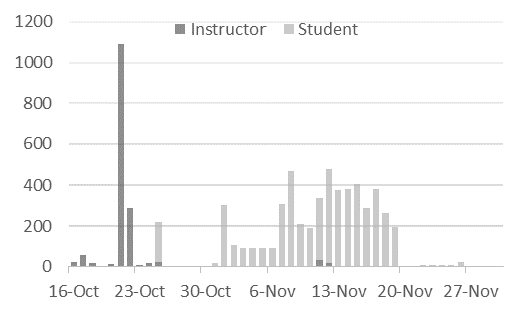
\includegraphics[width=1.0\columnwidth]{images/fig4.pdf} 
  \caption{Usage between instructors and students for vCPU cores}\label{F:fig5} 
\end{figure} 

For this class 25 hosts, with 216 vCPUs and 600GB memories were reserved as to satisfy the request of accessing large virtual instances. In Figure~\ref{F:fig6} we demonstrate that the dedicated resources were being underutilized most time although the high volume requests had been made including a 273\% overutilization on October 21th for testing and preparing. However, if the resources would have not been separated as part of its own cloud it would have been possible to allow resource aggregation and policy definitions that allow autoscaling in support of this class.
  
\begin{figure}[htb] 
  \centering 
    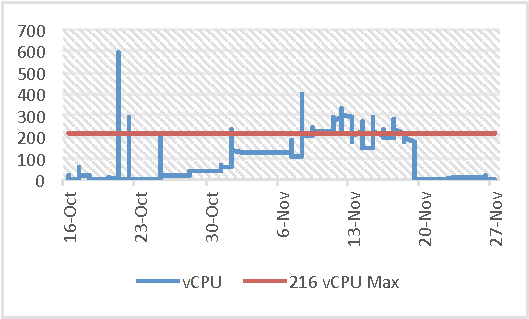
\includegraphics[width=1.0\columnwidth]{images/fig5.pdf} 
  \caption{vCPU Utilization (approximation per hour)}\label{F:fig6} 
\end{figure} 

High Performance Computing (HPC) has been used to support parallel data processing of big data. In Figure~\ref{F:bigdata} we see that in addition to IaaS big data projects have also requested HPC and other services. Additionally we can see that the initial dominant usage of Eucalyptus and Nimbus as IaaS has been replaced with OpenStack.  Toghether this data shows it is desirable to provide a hybrid cloud that integrates HPC and IaaS service to scientists and researchers.

\begin{figure}[htb]
  \centering
    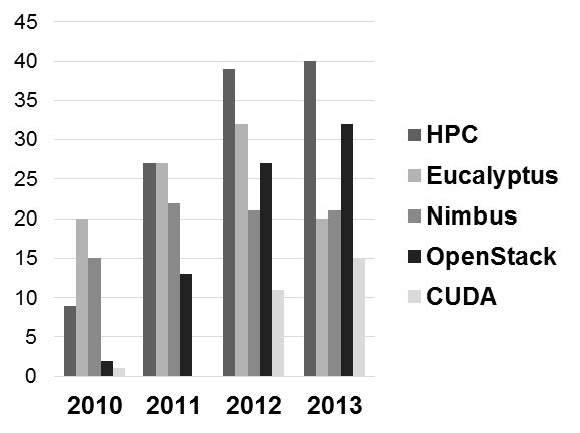
\includegraphics[width=1.0\columnwidth]{images/bigdata.pdf} 
  \caption{Service changes for along with Big Data between 2010 and 2013}\label{F:bigdata} 
\end{figure} 

Another important result was that the number of servers per job requested as part of HPC usage increased. We found that for HPC, 64 and 128 CPU cores per job are most popular job sizes in FutureGrid HPC in 2013 (See Figure~\ref{F:bigdatainhpc}). 24\% and 14\% of total wall time are for 64 and 128 cpu jobs. An extra large jobs (i.e. 512 CPU cores) has been intensively used in the last year. Compared to the previous year 2012, the request has been increased about 350\%. In early stage of FutureGrid between 2010 and 2011, tiny CPU jobs have been requested many times but in 2013, two thirds jobs are using more than 64 CPU cores. This shows the user community in FuturGrid matured using more servers at a time than before.

\begin{figure}[htb]
  \centering
    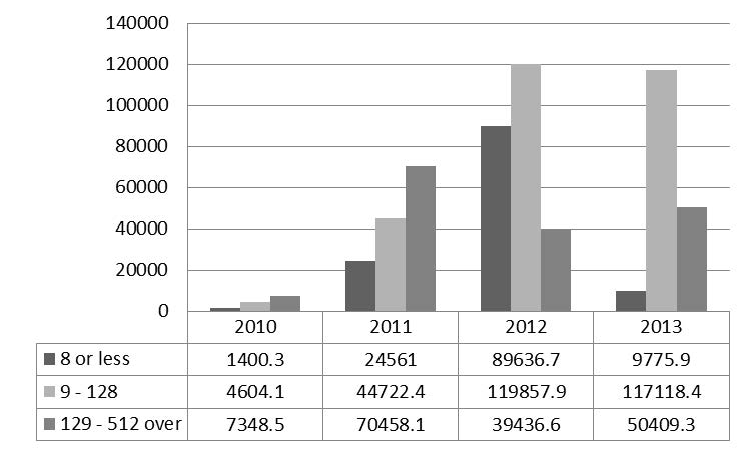
\includegraphics[width=1.0\columnwidth]{images/bigdatainhpc.pdf} 
  \caption{Annual Wall Time Changes for Job Size in HPC between 2010 and 2013}\label{F:bigdatainhpc} 
\end{figure} 

Clearly we see from our examples that valuable information can be derived already with the cloudmesh metrics framework. The ability to have access to standard reports makes reporting and oversight easier. Furthermore data we collected could be used to convince those that are used to exclusive use of resources in favor of shared cloud resources.

\begin{comment}

%%%%%%%%%%%%%%%%%%%%%%%%%%%%%%%%%%%%%%%%%%%%%%%%%%%%%%%%%%%%%%%%%%%%%% 
\section{PaaS Metrics}\label{S:paas}
%%%%%%%%%%%%%%%%%%%%%%%%%%%%%%%%%%%%%%%%%%%%%%%%%%%%%%%%%%%%%%%%%%%%%% 


http://blog.cobia.net/cobiacomm/2013/01/29/paas-performance-metrics/

Foundational PaaS performance metrics focus on time to market.  Key metrics include:

Time and effort to create new application environment
Time to redeploy application
Time to promote application into a new lifecycle phase

Optimization PaaS performance metrics focus on portfolio efficiency.  Key metrics include

Ability to dynamically right-size infrastructure and elastic scalability
Ability to re-use existing platform services and business services from resource pool instead of re-building solution stack

Transformational PaaS performance metrics focus on productivity.   Key metrics include:

Time and effort required integrating business process, event processor – creating a complex app.
Time and effort required to apply policy across tenant(s)
Cost to operate application per user or transaction measured against the value provided by the application or transaction.


----

http://thenewstack.io/heroku-rolls-out-metrics-to-help-users-optimize-performance/

\end{comment}

%%%%%%%%%%%%%%%%%%%%%%%%%%%%%%%%%%%%%%%%%%%%%%%%%%%%%%%%%%%%%%%%%%%%%% 
\section{RELATED WORK}\label{S:related}
%%%%%%%%%%%%%%%%%%%%%%%%%%%%%%%%%%%%%%%%%%%%%%%%%%%%%%%%%%%%%%%%%%%%%% 


\task{This section will contain some relevant related work. We have
  included a small set of references that may be helpful to establish
  this section. Right now we provide a list of unordered refernces}

Nist~\cite{NIST2015}
Blueflood~\cite{BlueFloodDB}
CM-measurement facets for cloud performance~\cite{singh2011cm}
Online detection of utility cloud anomalies using metric distributions~\cite{wang2010online}
M4Cloud-Generic Application Level Monitoring for Resource-shared Cloud Environments.~\cite{mastelic2012m4cloud}
Design of a Dynamic Provisioning System for a Federated Cloud and Bare-metal Environment~\cite{vondesign}
\cite{CloudAuditingDataFederation}
\cite{viewing-keystone-cadf-notifications-with-ceilometer-and-rabbitmq}
\cite{GoogleCustomMetrics}
\cite{terencengai}
\cite{KevinFogarty}
\cite{SharonWagner}
\cite{MarcusSarmento}
\cite{cloudwatch2013monitoring}
\cite{RobBoucher}
\cite{GregorBeslic}
\cite{aceto2013cloud}
\cite{HPHelionEucalyptus}
\cite{eucalyptusgithub}
\cite{ceilometer}
\cite{gcemonitoring}
\cite{securitymetrics}
\cite{securitymetrics-educause}

\subsection{Surveys and Taxonomies}

\task{This section will include a small survey of paper that provide
  them selfs surveys to cloud metrics.}

\cite{vineetha2012performance}
\cite{alhamazani2013overview}
\cite{fourkeys-for-monitoring}

\cite{aceto2012cloud}
\cite{clayman2010monitoring}
\cite{fatema2014survey}
\cite{paessler2012monitoring}
\cite{mohamaddiah2014survey}
\cite{brinkmann2013scalable}
\cite{gorbil2014principles}
\cite{ward2014observing}
\cite{danetwork}
\cite{petcu2014towards}
\cite{zhang2013survey}
\cite{smith2014building}

RightScale~\cite{rightscalereport13}


%%%%%%%%%%%%%%%%%%%%%%%%%%%%%%%%%%%%%%%%%%%%%%%%%%%%%%%%%%%%%%%%%%%%%%
\section{CONCLUSION}\label{S:conclusion}
%%%%%%%%%%%%%%%%%%%%%%%%%%%%%%%%%%%%%%%%%%%%%%%%%%%%%%%%%%%%%%%%%%%%%%

\task{write conclusion}


%%%%%%%%%%%%%%%%%%%%%%%%%%%%%%%%%%%%%%%%%%%%%%%%%%%%%%%%%%%%%%%%%%%%%% 
% Acknowledgment 
%%%%%%%%%%%%%%%%%%%%%%%%%%%%%%%%%%%%%%%%%%%%%%%%%%%%%%%%%%%%%%%%%%%%%% 
  
\section{ACKNOWLEDGEMENT} 
 
This material based upon work is partially supported in part by the National Science Foundation under Grant No. 1445806, 1445806, and 0910812.

\begin{scriptsize} 
\bibliographystyle{IEEEtranS} 
%\bibliographystyle{abbrv} 
\bibliography{%
bib/tas-dedup,%
bib/vonLaszewski-jabref,% 
bib/cyberaide-metric,%
bib/cyberaide-cloud,%
metric-new,%
bib/image-refs}
\end{scriptsize}
   
%bib/python,% 
%tas.bib%


\appendix

\section{XDMOD metrics compared to Cloud Metrics}

This appendix includes a number of tables that summarize metrics that are exposed by the XDMoD framework applied to XSEDE. We showcase the following:

\begin{description}

\item[Table \ref{T:xdmod}] shows \hyungro{complete}.
.
\item[Table \ref{T:xdmod2}] shows \hyungro{complete}.

\item[Table \ref{T:xdmod22}] shows \hyungro{complete}.

\item[Table \ref{T:xdmod23}] shows \hyungro{complete}.

\item[Table \ref{T:xdmod24}] shows \hyungro{complete}.

\item[Table \ref{T:xdmod3}] shows \hyungro{complete}.


\end{description}

\begin{table*}[htb]
  \caption{HPC Metric Categories in XDMoD}
\label{T:xdmod}
\begin{scriptsize}
\begin{tabular}{l|l|l} 
HPC Category & Compatibility with IaaS & Description\\
\hline
Job & VM & The number of requested jobs in HPC or VM instance in the cloud\\
Allocations & Project(Tenant) & A funded project that is allowed to run jobs (VMs) on resources \\
Accounts & Accounts & The number of user accounts registered or deleted \\
Requests & Requests & The number of registered projects or accounts\\
% Performance & Performance & TBD \\
% SUPREMM & - & TBD \\
\hline
\end{tabular}\\
\end{scriptsize}
\end{table*}



\begin{table*}[htb]
  \caption{Metrics Comparison between HPC and Cloud}
\label{T:xdmod2}

\begin{scriptsize}
\begin{tabular}{l|l|l} 
HPC Metric & IaaS Metric & Description \\
\hline
CPU Hours: Per Job  & vCPU Hours: Per VM & The average CPU hours per job or VM to measure CPU utilization \\
CPU Hours: Total  & vCPU Hours: Total & The total CPU hours for all jobs or VMs \\
Job Size: Max/Min  & vCPU Count: Total & The total number of processor cores ubsed by a job or a VM \\
Job Size: Normalized  & vCPU Count: Normalized & The percentage total number of processor cores used over the entire cores\\
Job Size: Per Job  & vCPU Count: Per VM & The number of processor cores per HPC job or VM instance\\
Node Hours: Per Job  & Node Hours: Per VM & The average compute node hours per HPC job or VM instance \\
Node Hours: Total  & Node Hours: Per VM & The total compute node hours used by HPC jobs or VM instances \\
Number of Jobs & Number of VMs & The total number of jobs or VMs with its status: Started/Running/Terminated\\
Number of Users & Number of Users & The total number of active users \\
Power (Electricity) & Power (Electricity) & The amount of energy used in HPC or the cloud by Kilo Watt per hour (KWh) \\
User Expansion Factor  & N/A & (HPC Only) job-turnaround time, 
((wait time + wall time) / wall time)\\
Wait Hours: Per Job  & N/A & (HPC Only) The average hours of waiting to run a job on the designated resource\\
Wait Hours: Total  & N/A & (HPC Only) The total hours of waiting to run jobs on the designated resource \\
Wall Hours: Per Job  & Running Hours: Per VM &  The average hours of running a job or a VM\\
Wall Hours: Total  & Running Hours: Per VM & The total hours of running jobs or VMs \\
N/A & IP Count: Public or Private & (Cloud Only) The total number of allocated public IP addresses \\
N/A & Storage Sizes: Block or Object & (Cloud Only) The total size of allocated storage sizes \\
% Allocation Usage Rate & TBD & The rate of XSEDE allocation usage in XD SUs per hour \\
% Job Size: Weighted By XD SUs  & TBD & TBD \\
% NUs Charged: Per Job  & TBD & TBD \\
% NUs Charged: Total  & TBD & TBD \\
% Number of Allocations: Active  & TBD & TBD \\
% Number of Institutions: Active  & TBD & TBD \\
% Number of PIs: Active  & TBD & TBD \\
% Number of Resources: Active  & TBD & TBD \\
% XD SUs Charged: Per Job  & TBD & TBD \\
% XD SUs Charged: Total  & TBD & TBD \\
% XSEDE Utilization  & TBD & TBD \\
\hline
\end{tabular}\\
\end{scriptsize}
\end{table*}


\begin{table*}[htb]
  \caption{Account related metrics in XDMoD}
\label{T:xdmod22}
\begin{scriptsize}
\begin{tabular}{l|l} 
Metric & Description \\
\hline
Number of User Accounts: Closed & TBD \\
Number of User Accounts: Created & TBD \\
Number of User Accounts: Open & TBD \\
\hline
\end{tabular}\\
\end{scriptsize}
\end{table*}

\begin{table*}[htb]
  \caption{HPC Performance related metrics in XDMoD}
\label{T:xdmod23}
\begin{scriptsize}
\begin{tabular}{l|l} 
Metric & Description \\
\hline
Avg IO Performance & TBD \\
Avg Memory Performance & TBD \\
Avg Network Performance & TBD \\
Avg System Performance & TBD \\
CPU:Graph500 - Performance & TBD \\
CPU:OSJitter - Inv Mean Noise & TBD \\
CPUIO:NWCHEM - Performance & TBD \\
CPUNET:HPCC - DGEMM & TBD \\
CPUNET:HPCC - FFTW & TBD \\
CPUNET:HPCC - LINPACK & TBD \\
CPUNET:NPB - BT & TBD \\
CPUNET:NPB - CG & TBD \\
CPUNET:NPB - FT & TBD \\
CPUNET:NPB - LU & TBD \\
CPUNET:NPB - MG & TBD \\
CPUNET:NPB - SP & TBD \\
IO:IOR - MPIIO Col Read & TBD \\
IO:IOR - MPIIO Col Write & TBD \\
IO:IOR - MPIIO Ind Read & TBD \\
IO:IOR - MPIIO Ind Write & TBD \\
IONET:MPI-Tile-IO - 3D Col Read & TBD \\
IONET:MPI-Tile-IO - 3D Col Write & TBD \\
Mem:HPCC - Bandwidth & TBD \\
Net:Graph500 - TEPS & TBD \\
Net:HPCC - MPI Random Access & TBD \\
Net:HPCC - PTRANS & TBD \\
\hline
\end{tabular}\\
\end{scriptsize}
\end{table*}

\begin{table*}[htb]
  \caption{2nd Category IV in XDMoD}
\label{T:xdmod24}

\begin{scriptsize}
\begin{tabular}{l|l} 
Metric & Description \\
\hline
Avg CPU \%: Idle: weighted by core-hour &  TBD \\
Avg CPU \%: System: weighted by core-hour &  TBD \\
Avg CPU \%: User: weighted by core-hour &  TBD \\
Avg: /home write rate: Per Node weighted by node-hour &  TBD \\
Avg: /scratch write rate: Per Node weighted by node-hour &  TBD \\
Avg: /work write rate: Per Node weighted by node-hour &  TBD \\
Avg: CPI: Per Core weighted by core-hour &  TBD \\
Avg: CPLD: Per Core weighted by core-hour &  TBD \\
Avg: CPU User CV: weighted by core-hour &  TBD \\
Avg: CPU User Imbalance: weighted by core-hour &  TBD \\
Avg: FLOPS: Per Core weighted by core-hour &  TBD \\
Avg: InfiniBand rate: Per Node weighted by node-hour &  TBD \\
Avg: Memory Bandwidth: Per Core weighted by core-hour &  TBD \\
Avg: Memory: Per Core weighted by core-hour &  TBD \\
Avg: Total Memory: Per Core weighted by core-hour &  TBD \\
Avg: block sda read ops rate: Per Node weighted by node-hour &  TBD \\
Avg: block sda read rate: Per Node weighted by node-hour &  TBD \\
Avg: block sda write ops rate: Per Node weighted by node-hour &  TBD \\
Avg: block sda write rate: Per Node weighted by node-hour &  TBD \\
Avg: eth0 receive rate: Per Node weighted by node-hour &  TBD \\
Avg: eth0 transmit rate: Per Node weighted by node-hour &  TBD \\
Avg: ib0 receive rate: Per Node weighted by node-hour &  TBD \\
Avg: ib0 transmit rate: Per Node weighted by node-hour &  TBD \\
Avg: lustre receive rate: Per Node weighted by node-hour &  TBD \\
Avg: lustre transmit rate: Per Node weighted by node-hour &  TBD \\
Avg: mic0 receive rate: Per Node weighted by node-hour &  TBD \\
Avg: mic0 transmit rate: Per Node weighted by node-hour &  TBD \\
Avg: mic1 receive rate: Per Node weighted by node-hour &  TBD \\
Avg: mic1 transmit rate: Per Node weighted by node-hour &  TBD \\
CPU Hours: Idle: Total &  TBD \\
CPU Hours: System: Total &  TBD \\
CPU Hours: Total &  TBD \\
CPU Hours: User: Total &  TBD \\
Number of Jobs Ended &  TBD \\
Number of Jobs Running &  TBD \\
Number of Jobs Started &  TBD \\
Number of Jobs Submitted &  TBD \\
Wait Hours: Per Job &  TBD \\
Wait Hours: Total &  TBD \\
Wall Hours: Per Job &  TBD \\
Wall Hours: Requested: Per Job &  TBD \\
Wall Hours: Requested: Total &  TBD \\
\hline 
\end{tabular}\\
\end{scriptsize}
\end{table*}


\begin{table*}[htb]
  \caption{Group By in XDMoD}
\label{T:xdmod3}

\begin{scriptsize}
\begin{tabular}{l|l} 
Group & Description \\
\hline
Summary & TBD \\
Allocation & TBD \\
Field of Science & The field of science indicated on the allocation request pertaining to the running job \\
Gateway & TBD \\
Grant Type & TBD \\
Job Size & TBD \\
Job Wall Time & TBD \\
Node Count & TBD \\
NSF Directorate & TBD \\
Parent Science & TBD \\
PI & TBD \\
PI Institution & TBD \\
Resource & TBD \\
Resource Type & TBD \\
Service Provider & TBD \\
System Username & TBD \\
User & TBD \\
User Institution & TBD \\
User NSF Status & TBD \\
\hline
\end{tabular}\\
\end{scriptsize}
\end{table*}


\end{document} 

%%%%%%%%%%%%%%%%%%%%%%%%%%%%%%%%%%%%%%%%%%%%%%%%%%%%%%%%%%%%%%%%%%%%%% 
% END DOCUMENT
%%%%%%%%%%%%%%%%%%%%%%%%%%%%%%%%%%%%%%%%%%%%%%%%%%%%%%%%%%%%%%%%%%%%%% 


\begin{comment}
Additional metrics that we have not yet included into the tables include the following

\begin{Verbatim}[fontfamily=times]
o monitoring service
  o errors
    - detect incidents
    - trace issues/ bugs
    - prevent long downtime
  - alert/notification (e.g. text, email)
  - diagnostics
  - security
  - capacity planning/prediction
  - trend changes
o audit/assurance
  - user behavior
\end{Verbatim}
\end{comment}

